%%%%%%%%%%%%%%%%%%%%%%%%%%%%%%%%%%%%%%%%%%%%%%%%%%%%%%%%%%
%   Vorlage von:
%
%   Prof. Dr. Bernhard Drabant
%   Prof. Dr. Dennis Pfisterer
%   Prof. Dr. Julian Reichwald
%
%%%%%%%%%%%%%%%%%%%%%%%%%%%%%%%%%%%%%%%%%%%%%%%%%%%%%%%%%%

%%%%%%%%%%%%%%%%%%%%%%%%%%%%%%%%%%%%%%%%%%%%%%%%%%%%%%%%%%
%	ANLEITUNG: 
%
%   1. Ersetzen Sie firmenlogo.jpg im Verzeichnis img
%   2. Passen Sie alle Stellen im Dokument an, die mit 
%      @stud markiert sind
%
%%%%%%%%%%%%%%%%%%%%%%%%%%%%%%%%%%%%%%%%%%%%%%%%%%%%%%%%%%

%%%%%%%%%%%%%%%%%%%%%%%%%%%%%%%%%%%%%%%%%%%%%%%%%%%%%%%%%%
%	ACHTUNG: 
%
%   Für das Erstellen des Literaturverzeichnisses wird das 
%   modernere Paket biblatex in Kombination mit biber 
%   verwendet -- nicht mehr das ältere BibTex!
%   Bitte stellen Sie ggf. Ihre TeX-Umgebung entsprechend 
%   ein (z.B. TeXStudio: Einstellungen --> Erzeugen --> 
%   Standard Bibliographieprogramm: biber)
%
%%%%%%%%%%%%%%%%%%%%%%%%%%%%%%%%%%%%%%%%%%%%%%%%%%%%%%%%%%

\documentclass[fontsize=12pt,BCOR=5mm,DIV=12,
               parskip=half,
               listof=entryprefix,paper=a4,toc=bibliography,toc=listof,pointlessnumbers,ngerman
               %,headinclude=on,footinclude=off,
               %,plainheadtopline=false,plainheadsepline=false,plainfootsepline=false,plainfootbotline=false
               ]{scrreprt}
               
\makeindex

% (!!) Elementare Pakete, Konfigurationen und Definitionen werden geladen
% !TEX root =  master.tex
%      HYPERREF

%%%%%%%%%%%%%%%%%%%%%%%%%%%%%%%%%%%%%%%%%%%%%%%%%%%%%%%%%%
%	ANLEITUNG: 
%
% Passen Sie alle Stellen im Dokument an, die mit 
% @stud markiert sind
%
%%%%%%%%%%%%%%%%%%%%%%%%%%%%%%%%%%%%%%%%%%%%%%%%%%%%%%%%%%

\usepackage{makeidx}         % allows index generation
\usepackage{listings}	%Format Listings properly
\usepackage{lipsum}    %Blindtext
\usepackage{graphicx} % use various graphics formats
\usepackage[german]{varioref} 	% nicer references \vref
\usepackage{caption}	%better Captions
\usepackage{booktabs} %nicer Tabs
\usepackage{array}
\usepackage{chngcntr}
\usepackage[hidelinks=true]{hyperref} % keine roten Markierungen bei Links
\usepackage{fnpct} % Correct superscripts 
\usepackage[T1]{fontenc}
\usepackage[utf8]{inputenc}
\usepackage{calc} % Used for extra space below footsepline
\usepackage{acronym}
\usepackage{algorithm}
\usepackage{algpseudocode}
\usepackage{setspace}

%
% @stud
%
%	FONT SELECTION: Entweder 1) Latin Modern oder 2) Times / Helvetica
\usepackage{lmodern}             % 1) Latin modern font
%\usepackage{mathptmx}           % 2) Helvetica / Times New Roman fonts (2 lines)
%\usepackage[scaled=.92]{helvet} % 2) Helvetica / Times New Roman fonts (2 lines)

%
% @stud
%
%	LANGUAGE SETTINGS
\usepackage[ngerman]{babel} 	        % german language
\usepackage[german=quotes]{csquotes} 	% correct quoting using \enquote{}
%\usepackage[english]{babel}          % english language
%\usepackage{csquotes} 	              % correct quoting using \enquote{}

%
% @stud
%
% Uncomment the following lines to support hard URL breaks in bibliography 
%\apptocmd{\UrlBreaks}{\do\f\do\m}{}{}
%\setcounter{biburllcpenalty}{9000}% Kleinbuchstaben
%\setcounter{biburlucpenalty}{9000}% Großbuchstaben

%
% @stud
%
%	FOOTNOTES: Count footnotes over chapters
%1 \counterwithout{footnote}{chapter}

%	ACRONYMS
\makeatletter
\@ifpackagelater{acronym}{2015/03/20}
{\renewcommand*{\aclabelfont}[1]{\textbf{{\acsfont{#1}}}}}{}
\makeatother

%	LISTINGS
\renewcommand{\lstlistingname}{Quelltext} 
\renewcommand{\lstlistlistingname}{Quelltextverzeichnis}
\lstset{numbers=left,
	numberstyle=\tiny,
	captionpos=b,
	basicstyle=\ttfamily\small}

%	ALGORITHMS
\renewcommand{\listalgorithmname}{Algorithmenverzeichnis }
\floatname{algorithm}{Algorithmus}

%		PAGE HEADER / FOOTER
%	    Warning: There are some redefinitions throughout the master.tex-file!  DON'T CHANGE THESE REDEFINITIONS!
\RequirePackage[automark]{scrlayer-scrpage}
%alternatively with separation lines: \RequirePackage[automark,headsepline,footsepline]{scrlayer-scrpage}

%\renewcommand*{\pnumfont}{\upshape\sffamily}
%\renewcommand*{\headfont}{\upshape\sffamily}
%\renewcommand*{\footfont}{\upshape\sffamily}

\renewcommand{\chaptermarkformat}{}
\RedeclareSectionCommand[beforeskip=0pt]{chapter}
\clearscrheadfoot

%\ifoot[\rule{0pt}{\ht\strutbox+\dp\strutbox}DHBW Mannheim]{\rule{0pt}{\ht\strutbox+\dp\strutbox}DHBW Mannheim}
\ofoot[\rule{0pt}{\ht\strutbox+\dp\strutbox}\pagemark]{\rule{0pt}{\ht\strutbox+\dp\strutbox}\pagemark}
\ohead{\headmark}

\newcommand{\TitelDerArbeit}[1]{\def\DerTitelDerArbeit{#1}\hypersetup{pdftitle={#1}}}
\newcommand{\AutorDerArbeit}[1]{\def\DerAutorDerArbeit{#1}\hypersetup{pdfauthor={#1}}}
\newcommand{\Firma}[1]{\def\DerNameDerFirma{#1}}
\newcommand{\Kurs}[1]{\def\DieKursbezeichnung{#1}}
\newcommand{\Abteilung}[1]{\def\DerNameDerAbteilung{#1}}
\newcommand{\Studiengangsleiter}[1]{\def\DerStudiengangsleiter{#1}}
\newcommand{\WissBetreuer}[1]{\def\DerWissBetreuer{#1}}
\newcommand{\FirmenBetreuer}[1]{\def\DerFirmenBetreuer{#1}}
\newcommand{\Bearbeitungszeitraum}[1]{\def\DerBearbeitungszeitraum{#1}}
\newcommand{\Abgabedatum}[1]{\def\DasAbgabedatum{#1}}
\newcommand{\Matrikelnummer}[1]{\def\DieMatrikelnummer{#1}}
\newcommand{\Studienrichtung}[1]{\def\DieStudienrichtung{#1}}
\newcommand{\ArtDerArbeit}[1]{\def\DieArtDerArbeit{#1}}
\newcommand{\Literaturverzeichnis}{Literaturverzeichnis}

\newcommand{\settingBibFootnoteCite}{
	\setlength{\bibparsep}{\parskip}		  % Add some space between biblatex entries in the bibliography
	\addbibresource{bibliography.bib}	    % Add file bibliography.bib as biblatex resource
	\DefineBibliographyStrings{ngerman}{andothers = {{et\,al\adddot}},}
	\AdaptNoteOpt\footcite\multfootcite   % Will add  separators if footcite is called multiple consecutive times 
	\AdaptNoteOpt\autocite\multautocite   % Will add  separators if autocite is called multiple consecutive times
}

\newcommand{\setTitlepage}{
	% !TEX root =  master.tex
\begin{titlepage}
	\begin{center}
		
\includegraphics[width=8cm]{\imagedir/logo.jpg}	
	\end{center}
	\vspace{2em}
	%\sffamily
	\begin{center}
		{\textsf{\large Duale Hochschule Baden-W\"urttemberg Mannheim}}\\[4em]
		{\textsf{\textbf{\large{\DieArtDerArbeit}arbeit}}}\\[6mm]
		{\textsf{\textbf{\Large{}\DerTitelDerArbeit}}} \\[1.5cm]
		{\textsf{\textbf{\large{}Studiengang Wirtschaftsinformatik}}\\[6mm]
		\textsf{\textbf{Studienrichtung \DieStudienrichtung}}}\\[6mm]
		\textsf{Kurs: \DieKursbezeichnung} \\[1.5cm]

		\textbf{\href{https://github.com/DHBWMannheim/learninganalystics/}{Quellcode}
		-
		\href{https://dhbwlearning.web.app/}{Website}}


		\vspace{1.5cm}

		\begin{center}
			\begin{table}[h]
				\centering
				\begin{tabular}{c}
					Aaron Schweig \\
					Jan Grübener \\
					Matthias Vonend  \\
					Michael Angermeier \\
					Patrick Mischka \\
					Troy Kessler \\
				\end{tabular}
			\end{table}
		\end{center}

		% \begin{minipage}{\textwidth}
		% 	\begin{tabbing}
		% 		Bearbeitungszeitraum: \hspace{0.85cm}\=\kill
		% 		% TODO: Verfasser
		% 		Kurs: \> \DieKursbezeichnung \\[1.5mm]
		% 		Bearbeitungszeitraum: \> \DerBearbeitungszeitraum\\[1.5mm]
		% %		alternativ:\\[1.5mm]
		% %		Eingereicht: \> \DasAbgabedatum	
		% 	\end{tabbing}
		% \end{minipage}
	\end{center}
\end{titlepage}
	\pagenumbering{roman} % Römische Seitennummerierung
	\normalfont	
}

%
% @stud
%
\newcommand{\settingLists}{
	%	Inhaltsverzeichnis
	\tableofcontents
	%	Abbildungsverzeichnis
	\listoffigures
	%	Tabellenverzeichnis
	\listoftables
	%	Listingsverzeichnis / Quelltextverzeichnis
	\lstlistoflistings
	% Algorithmenverzeichnis
	\listofalgorithms
}

\newcommand{\initializeText}{
	\clearpage
	\ihead{\chaptername~\thechapter} % Neue Header-Definition
	\pagenumbering{arabic}           % Arabische Seitenzahlen
}

\newcommand{\initializeBibliography}{
	\ihead{}
	\printbibliography[title=\Literaturverzeichnis] 
	\cleardoublepage
}

\newcommand{\initializeAppendix}{
	\appendix
	\ihead{\appendixname~\thechapter}
}



%%%%%%%%%%%%%%%%%%%%%%%%%%%%
%
% @stud
%
%	SCHRIFTART (Schrift mit oder ohne Serifen im gesamten Text) 
%
% mit Serifen
%\addtokomafont{disposition}{\rmfamily}
%\renewcommand*{\familydefault}{\rmdefault}
%
% ohne Serifen (default)
%\addtokomafont{disposition}{\sffamily}
%
%%%%%%%%%%%%%%%%%%%%%%%%%%%%

%%%%%%%%%%%%%%%%%%%%%%%%%%%%
%
% @stud
%
% PERSÖNLICHE ANGABEN (BITTE VOLLSTÄNDIG EINGEBEN zwischen den Klammern: {...})
%
\ArtDerArbeit{Studien} % "Bachelor" oder "Projekt" wählen
\TitelDerArbeit{Learninganalystics}
\Kurs{WWI18SEA/C}
\Studienrichtung{Software Engineering}

\newcommand{\NameDerAnwendung}[0]{\enquote{DHBW Learning}} 
%
%%%%%%%%%%%%%%%%%%%%%%%%%%%%

%%%%%%%%%%%%%%%%%%%%%%%%%%%%
%
% @stud
%
%	BIBLIOGRAPHY (@stud: Bibliographie-Stil wählen - Position und Indizierung)
%
% Auswahl zwischen: IEEE Style, ALPHABETIC Style, HARVARD Style, AUTHOR-YEAR Style 
%
% (oder eigenen zulässigen Stil wählen) 
%

% Position des Zitats
%
\newcommand{\position}{inline} 
%\newcommand{\position}{footnote}

% Indizierung des Zitats
%
% 1) NUMERIC Style - e. g. [12]
\newcommand{\indextype}{numeric} 
%
% 2) ALPHABETIC Style - e. g. [AB12]
%\newcommand{\indextype}{alphabetic} 
%
% 3) IEEE Style - numeric kind of style 
%\newcommand{\indextype}{ieee} 
%
% 4) HARVARD Style 
%\newcommand{\indextype}{apa} 
%
% 5) CHICAGO Style 
%\newcommand{\indextype}{authoryear}
%
%%%%%%%%%%%%%%%%%%%%%%%%%%%%

\renewcommand*{\familydefault}{\sfdefault}

% \usepackage[backend=biber, autocite=\position, style=\indextype]{biblatex} 	

% \settingBibFootnoteCite

\newcommand{\abs}{\par\vskip 0.2cm\goodbreak\noindent}
\newcommand{\nl}{\par\noindent}
\newcommand{\mcl}[1]{\mathcal{#1}}
\newcommand{\nowrite}[1]{}
\newcommand{\NN}{{\mathbb N}}

\newcommand{\imagedir}{img}

\makeindex

\begin{document}

\setTitlepage

%%%%%%%%%%%%%%%%%%%%%%%%%%%%%%%%%%%%%%%%%%%%%%%%%%%%%%%%%%%%%%%%%%%%%%%%%%%%%%%%%%%%%%%%%%
% KAPITEL UND ANHÄNGE
%
% @stud:
%   - nicht benötigte: auskommentieren/löschen
%   - neue: bei Bedarf hinzufügen mittels input-Kommando an entsprechender Stelle einfügen
%%%%%%%%%%%%%%%%%%%%%%%%%%%%%%%%%%%%%%%%%%%%%%%%%%%%%%%%%%%%%%%%%%%%%%%%%%%%%%%%%%%%%%%%%%

%%%%%%%%%%%%%%%%%%%%%%%%%%%%%%%%%%%
% EHRENWÖRTLICHE ERKLÄRUNG
%
% @stud: ewerkl.tex bearbeiten
%
% % !TEX root =  master.tex
\clearpage
\chapter*{Ehrenwörtliche Erklärung}

% Wird die folgende Zeile auskommentiert, erscheint die ehrenwörtliche
% Erklärung im Inhaltsverzeichnis.

% \addcontentsline{toc}{chapter}{Ehrenwörtliche Erklärung}
Wir versichern hiermit, dass wir die vorliegende Arbeit mit dem Titel ``\textit{\DerTitelDerArbeit}'' selbstständig verfasst und keine anderen als die angegebenen Quellen und Hilfsmittel benutzt haben.

\vspace{3cm}
Ort, Datum \hfill 

 
%%%%%%%%%%%%%%%%%%%%%%%%%%%%%%%%%%%

%%%%%%%%%%%%%%%%%%%%%%%%%%%%%%%%%%%
% SPERRVERMERK
%
% @stud: nondisclosurenotice.tex bearbeiten
%
% \input{nondisclosurenotice} 
%%%%%%%%%%%%%%%%%%%%%%%%%%%%%%%%%%%

%%%%%%%%%%%%%%%%%%%%%%%%%%%%%%%%%%%
%	KURZFASSUNG
%
% @stud: acknowledge.tex bearbeiten
%
% \input{acknowledge} 
%%%%%%%%%%%%%%%%%%%%%%%%%%%%%%%%%%%

%%%%%%%%%%%%%%%%%%%%%%%%%%%%%%%%%%%
%	KURZFASSUNG
%
% @stud: abstract.tex bearbeiten
%
% !TEX root =  master.tex
\chapter*{Kurzfassung}

Hier können Sie die Kurzfassung (engl.~Abstract) der Arbeit schreiben. Beachten Sie dabei die Hinweise zum Verfassen der Kurzfassung.


 
%%%%%%%%%%%%%%%%%%%%%%%%%%%%%%%%%%%

%%%%%%%%%%%%%%%%%%%%%%%%%%%%%%%%%%%
% VERZEICHNISSE
%
% @stud: ggf. nicht benötigte Verzeichnisse auskommentieren/löschen in Def. von \settingLists in config.tex
%
\settingLists
%%%%%%%%%%%%%%%%%%%%%%%%%%%%%%%%%%%

%%%%%%%%%%%%%%%%%%%%%%%%%%%%%%%%%%%
% ABKÜRZUNGSVERZEICHNIS
%
% @stud: acronyms.tex bearbeiten
%
% !TEX root =  master.tex
\clearpage
\chapter*{Abkürzungsverzeichnis}	
\addcontentsline{toc}{chapter}{Abkürzungsverzeichnis}

\begin{acronym}[XXXXXXX] %TODO: Sortieren
	\acro{API}[API]{Application Programming Interface}
	\acro{BaaS}[BaaS]{Backend as a Service}
	\acro{IaaS}[IaaS]{Infrastructure as a Service}
	\acro{CaaS}[CaaS]{Container as a Service}
	\acro{FaaS}[FaaS]{Function as a Service}
	\acro{SaaS}[SaaS]{Software as a Service}
	\acro{MVC}[MVC]{Model-View-Controller}
	\acro{GUI}[GUI]{Graphical User Interface}
	\acro{UX}[UX]{User Experience}
	\acro{SLA}[SLA]{Service Level Agreement}
	\acro{RDB}[RDB]{Relational Database}
	\acro{CD}[CD]{Continuous Deployment}
	\acro{CI}[CI]{Continuous Integration}
	\acro{LMS}{Learning Management System}
\end{acronym} 
%%%%%%%%%%%%%%%%%%%%%%%%%%%%%%%%%%%

\initializeText
\onehalfspacing

%%%%%%%%%%%%%%%%%%%%%%%%%%%%%%%%%%%
% KAPITEL
%
% @stud: einzelne Kapitel bearbeiten und eigene Kapitel hier einfügen
%
% Einleitung
% !TEX root =  master.tex
\chapter{Einleitung}
\section{Motivation und Zielsetzung}
In den letzten Jahren hat Computertechnologie rasant an Leistungsfähigkeit und Funktionsumfang zugenommen.
Längst sind Computer oder Mobilgeräte nicht mehr aus dem Alltag wegzudenken.
Umso wichtiger ist es, diese Technologien sinnvoll in die Tätigkeiten von Menschen zu integrieren und so einen wertvollen Mehrwert zu generieren.
Immer mehr Themenbereiche sind und müssen digitalisiert werden.

Mit Blick auf das aktuelle Weltgeschehens sehen wir die Notwendigkeit, solche Technologien auch in den Hochschul-Kontext einzubringen.
Die aktuelle \enquote{Corona-Krise} hat extreme Auswirkungen und macht sich in vielen Bereichen bemerkbar.
Mit einer der Bereiche, die am stärksten betroffen sind, ist das Bildungswesen.
So sind bereits im April 2020 die Schulen von 192 Ländern geschlossen worden.\autocite[S. 845]{Donohue2020}
Die geänderten Anforderungen an Schüler und Studenten durch neue Konzepte wie \enquote{Home-Schooling} erfordern auch Anpassungen im Hochschulkontext.

Mit der von uns entwickelten Anwendung beabsichtigen wir die entstandene Distanz zwischen Studenten und Dozenten zu verringern. 
Mithilfe unserer Webanwendung möchten wir allen Studierenden und Dozierenden an der DHBW eine Möglichkeit bieten, ihren Hochschulalltag zu organisieren. 
Unsere Vision ist, dass durch unsere Anwendung ein Mehrwert für Studierende und Dozenten generiert wird.
Daher sollen möglichst alle Aufgaben des Hochschulalltags mit unserer Webanwendung unterstützt werden. 
Im Rahmen dieses Moduls soll ein Grundstein gelegt werden, auf dem weitere Entwicklung aufgebaut werden kann und auch soll.

\clearpage
\section{Aufbau der Arbeit} % TODO: Dieses Kapitel anpassen
In dieser Arbeit werden zunächst die Anforderungen an eine solche Anwendung betrachtet.
Dafür wird als erstes das Thema dieses Projektes abgegrenzt, um den Fokus unseres Vorhabens ausführlich darzustellen.
Anschließend wird der aktuelle Ist-Zustand analysiert um herauszufinden, wie Studenten und Dozenten am besten unterstützt werden können.
Ziel ist es festzustellen, welche funktionalen und welche nicht-funktionalen Anforderungen durch die Anwendung erfüllt werden sollten.

Basierend auf den festgestellten Anforderungen wird ein Konzept ausgearbeitet.
Im Konzept wird nicht nur auf die Funktionalitäten, wie sie Nutzer verwenden können, eingegangen, sondern auch auf die technischen Hintergründe.

Anschließend wird die Umsetzung des Konzeptes beschrieben.
Der Fokus liegt dabei auf der Schaffung von Transparenz bezogen auf die verarbeiteten Daten.
Als letztes Hauptkapitel wird die Nutzung der Anwendung durch dritte Personen wie Studenten und Dozenten beschrieben.
% TODO: Hier noch schauen. Soll die Nutztung tatsächlich als eigenes Kapitel geschrieben werden? ist das nicht schon in der Konzeption, und Umsetzung?

Das Nutzerhandbuch stellt eine eindeutige und verständliche Nutzeranleitung dar.
Mithilfe dieser werden alle Funktionalitäten der Endanwendung erklärt.
% TODO: Das auchnochmal reinschauen.   Brauchen wir wirklich ein Kapitel in dem nochmal die ganzen Anforderungen validiert werden? Das steht doch dann auch schon in Konzeption + Umsetzung ?
% TODO: Hier nochmal sätze bauen

Abschluss der Dokumentation ist die Zusammenfassung.
Diese besteht aus zwei Teilen.
Das Fazit betrachtet das Projekt als Ganzes und vergleicht die schlussendliche Form mit den in der Einleitung vorgestellten Zielen. Damit werden alle Tätigkeiten innerhalb dieses Projekts abgerundet und abgeschlossen dargestellt.
Anschließend wird ein Ausblick gegeben, an welchen Stellen Folgeprojekte aufbauen könnten, was wir aus aktueller Sicht als sinnvoll erachten würden, auf was dabei zu achten wäre und was vermieden werden sollte.


% TODO: Hier stand noch was drin, dass auch Datenschutz sachen und so beschrieben. Das weiß ich nicht. Das kann man hier reinschreiben, wenn wir das tatsächlich machen. 

\clearpage
\section{Vorgehen}
Wir haben uns in dieser Arbeit stark an das Vorgehen des Framworks Scrum gehalten. Scrum ist ein Vorgehensmodell aus der agilen Softwareentwicklung und dem agilen Projektmanagement. Das Framework vertritt die weit verbreitete Meinung, dass Softwareprojekte nicht im Voraus planbar sind, weshalb Planung nur schrittweise und durch immer weitere Verfeinerungen erfolgen sollte. Scrum basiert auf folgenden vier Grundwerten:
\begin{center}
	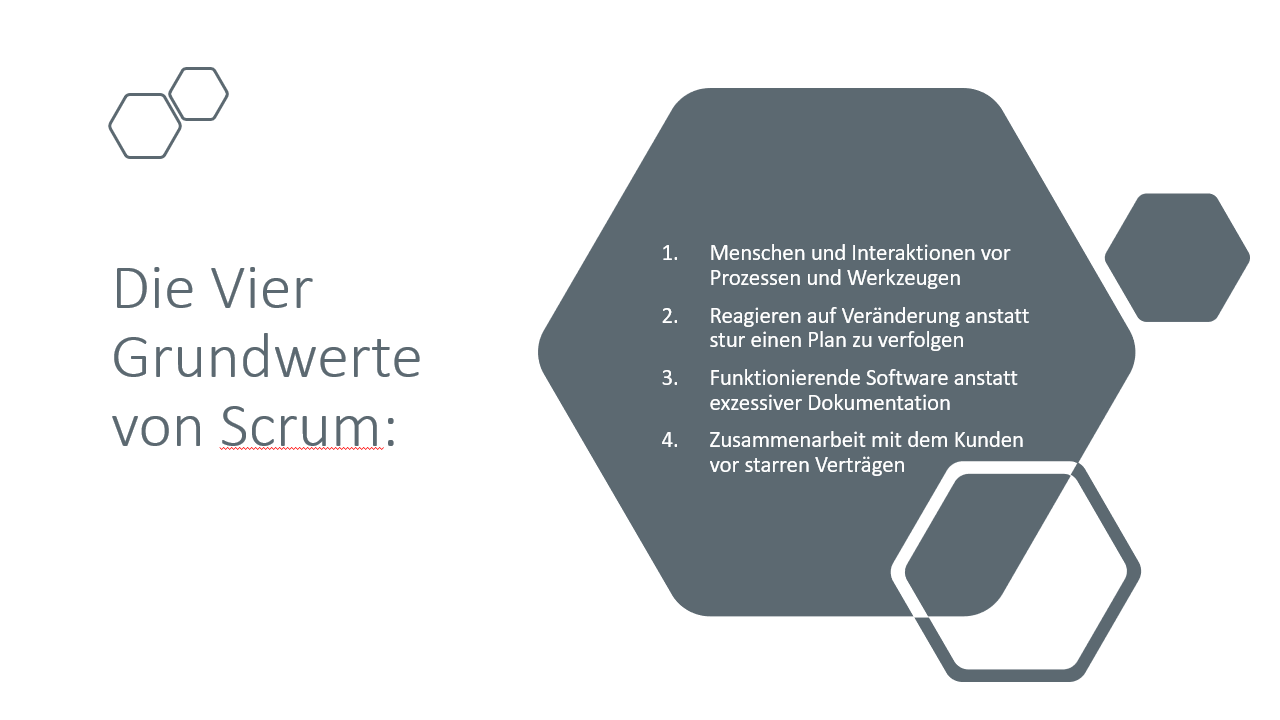
\includegraphics[width=14cm, keepaspectratio]{img/4Scrum} 
\end{center}

Wie bereits in der Beschreibung angeklungen ist, ist Scrum ein iteratives Vorgehen. Das beutetet, es gibt regelmäßige Arbeitsroutinen, die immer wiederholt werden. Ein solcher Abschnitt wird in Scrum Sprint genannt. Ein Sprint besteht aus folgenden festen Ritualen:
\begin{center}
	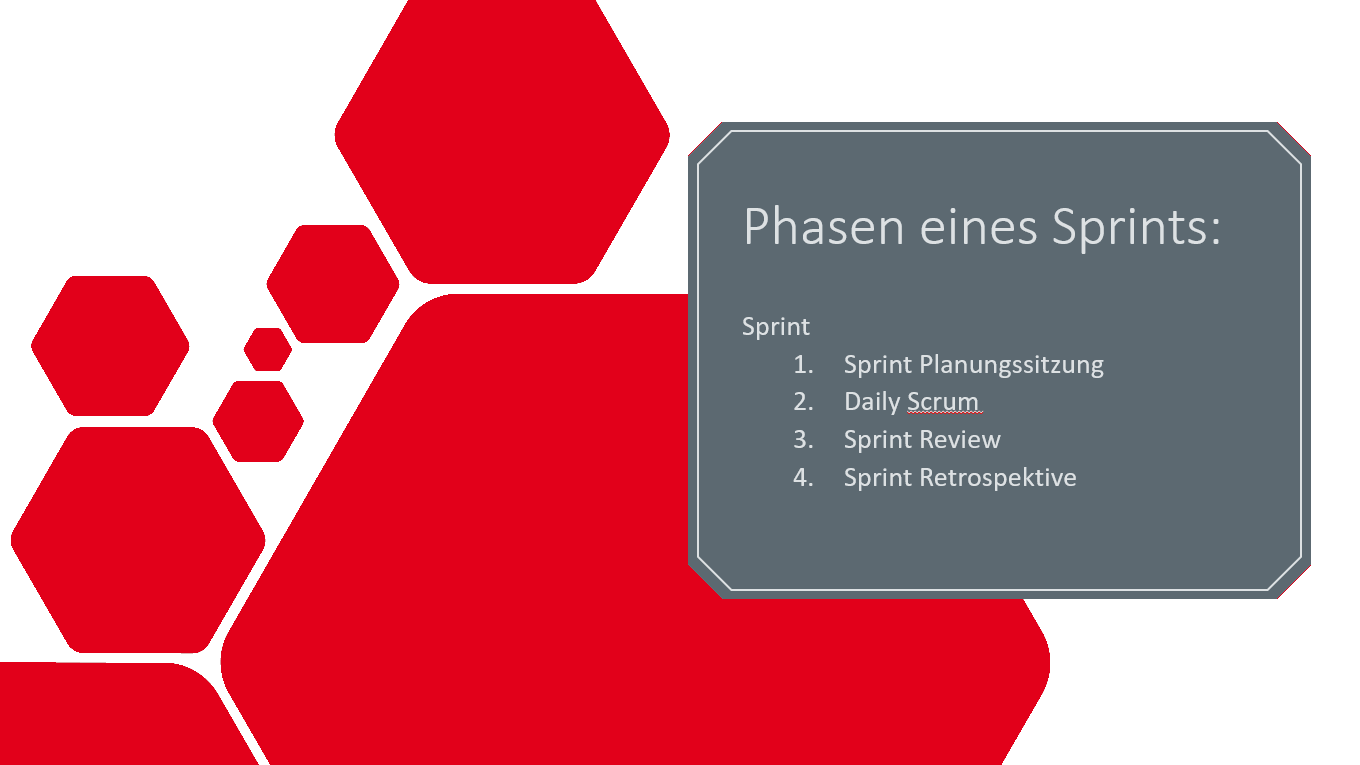
\includegraphics[width=14cm, keepaspectratio]{img/5Scrum} 
\end{center}


Wir haben uns für die Dauer eines Sprints von 2 Wochen entschieden. Zu Beginn eines jeden Sprints fand eine virtuelle Planungssitzung statt, bei der die anstehenden Aufgaben bezüglich ihrer Komplexität geschätzt wurden. In gemeinsamer Diskussion wurde entschieden, welche Aufgaben im Sprint erledigt und somit in das Sprint Backlog aufgenommen werden müssen. Da sich die Ausarbeitung dieses Projektes über zwei Theoriesemester und eine Praxisphase zog, in der wir auch unsere Bachelorarbeiten geschrieben haben, hatten wir uns schnell für das Pull Prinzip entschieden. Das bedeutet im Wesentlichen nur, dass jeder sich selbst Aufgaben annimmt und diese nicht zentral von einer Person zugewiesen bekommt. So wollten wir sicherstellen, dass jeder von uns zu jeder Zeit ein machbares Arbeitspensum erreichen konnte, bei dem wir zeitlich sowohl den Anforderungen des Projektes als auch den Vorberitungen für die zu schreibenden Klausuren und unseren Bachelorarbeiten  gerecht werden konnten. Die anfallenden Aufgaben haben wir in Arbeitspackete als Issues in unserem github Projekt angelegt, über das wir auch unseren Code versionierten und Deployments mittels github Actions anstießen. Ein Issue konnte prinzipiell jedes Team-Mitglied erstellen. Da innerhalb eines Sprints der Umfang und die Inhalte jedoch geschützt waren  und somit nicht verändert werden konnten, war sichergestellt, dass wir spätestens im nächsten Sprint Planning über diese Issues diskutieren, wenn es um die Frage ging, welche Inhalte im nächsten Sprint umgesetzt werden sollten.

 Das Daily Scrum Meeting stellte einen täglichen Termin dar, bei dem der aktuelle Stand der einzelnen Teammitglieder durchgegangen und gemeinsam über Probleme und Impediments gesprochen wurde. Aufgrund des langen Projektzeitraums und der oben genannten Gründe haben wir uns gegen ein tägliches Daily entschieden. Wir sind auch außerhalb des Sprintplannings regelmäßig in Kontakt und können so zielgerichteter und bedarfsgesteuert Themen in großer oder kleiner Gruppe diskutieren. 
 
 Ein Sprint Review fand am Ende eines jeden Sprints, also alle 14 Tage statt. Dabei wurden die umgesetzten Inhalte kurz der Gruppe vorgestellt und Feedback der Teammitglieder eingeholt. So konnten fachliche Missverständnisse schnell entdeckt und behoben werden. Außerdem verbesserte dieses Vorgehen im Regelfall die Codequalität. Scrum sieht eigentlich vor, das in diesem Termin auch die Stakeholder eingebunden werden, um Feedback der Auftraggeber frühestmöglich einholen zu können. Da dies aus Zeit- und Ressourcen-Gründen unrealistisch erschien, haben wir uns gemeinsam entschieden an dieser Stelle vom Prozess abzuweichen und nur die während den Vorlesungsstunden einberaumten Abstimmungen zu nutzen, um die seit der jeweils letzten Abstimmung umgesetzten Features vorzustellen und das weitere Vorgehen abzustimmen. Mit dieser Entscheidung haben wir uns auch verpflichtet, keine extra Sprint Retrospektive abzuhalten. Ziel dieses Termins ist es, innerhalb des Teams zu schauen, wie der letzte Sprint lief und wie man die gemeinsame Arbeit verbessern könnte. Dies wird üblicherweise  als extra Termin geplant, weil er dem Sprintteam gehört und nur intern bleiben soll. Hier gibt es in der Literatur sehr viele Beispiele auf die sogenannte Las Vegas Regel - \enquote{Alles was in Vegas passiert bleibt in Vegas}. 
 Da aber bereits unsere Sprint Reviews nur innerhalb des Teams abgehalten wurden beschlossen wir, nicht noch mehr Zeit für einem extra Termin aufwenden zu müssen, sondern in unserer speziellen Konstellation die beiden Termine nacheinander mit einem fließenden Übergang abzuhalten. 
 
Diesen Prozess verfolgten wir nach der ersten Vorlesung, die wir dazu nutzten, uns einen Überblick über die eigentliche Aufgabenstellung, das Themengebiet und die Arbeitspakete zu verschaffen. 

% mehrere Grundlagen- und Forschungs-Kapitel
% !TEX root =  ../master.tex
\chapter{Grundlage} % TODO: Kein Plan wo das hingehört
\section{Theoretische Grundlagen - Learning Analytics}

% TODO 2.1.2 Abgrenzungen zu anderen Anwendungen beachten
\subsection{Darlegung des Learning Analytics Konzepts}

%Begriff: Learning Analytics System 
Ein \ac{LMS} hat die grundlegenden Aufgaben Lernaktivitäten zu verwalten, aufzuzeichnen und über diese zu berichten. Diese \ac{LMS} können aus unterschiedlichsten Komponenten bestehen, die sich mit verschiedenen Aspekten dieser Aufgaben befassen \autocite[S.1]{learningManagementSystemsFieldGuide}. Zusätzlich sind entsprechende Nutzerdaten von Studierenden und Dozierenden zusammen mit den dazugehörigen Lernmaterialien innerhalb des \ac{LMS} zu verwalten \autocite{learningManagementSystemDefinition}\\
In einer Arbeit von 2013 \autocite[S.253]{SCHOONENBOOM2014247} sind verschiedene Formen von potentiellen Lernaktivitäten bei der Verwendung eines \ac{LMS} vorgestellt und im Rahmen einer Befragung von Studenten und Dozenten ausgewertet worden. Als entscheidende Einflüsse für Lernaktivitäten sind hierbei \enquote{Präsentationen}, \enquote{Referenzen auf weiterführende Inhalte}, \enquote{Fragemöglichkeiten für Studierende}, \enquote{hilfreiche Youtube-Inhalte} und \enquote{Feedbackmöglichkeiten von Dozenten} erkannt.

In der selben Arbeit \autocite[S.247]{SCHOONENBOOM2014247} wird auf die drei verschiedenen Ebenen von Leingegangen, welche Lernaktivitäten und deren Kontext darstellen.
\begin{enumerate}
	\item Auf der ersten Ebene befinden sich Werkzeuge (eng. \enquote{Tools}). Diese stellen konkrete Handlungen dar. Zum Beispiel könnte das Halten von Online-Vorlesungen ein Werkzeug darstellen.
	\item Auf der zweiten Ebene kann mit einem Werkzeug eine Lehr-/Unterrichtsaufgabe (eng. \enquote{instructional task}) unterstützt, beziehungsweise realisiert werden. Beispielsweise können gehaltene Online-Vorlesungen die Unterrichtsaufgabe realisieren, dass Studierenden Lehrinhalte erklärend vorgestellt werden.
	\item Die dritte Ebene stellt letztendlich konkrete Lernaktivitäten dar. Diese können durch eine Kombination von einer oder mehrere Lehr-/ Unterrichtsaufgaben erreicht werden. Um das Beispiel abzuschließen können in einer Online-Vorlesung (Werkzeug) vorgestellte Lerninhalte (Unterrichtsaufgabe) ein Lernaktivität induzieren, nämlich, dass aufmerksame Studierende die behandelten Themen der gehaltenen Vorlesung verstehen.	
\end{enumerate}

Aus all diesen Aktivitäten rund um \ac{LMS}, und im speziellen um Lernaktivitäten, lassen sich Daten erheben, die das Verhalten von Lehrenden und Lernenden darstellbar machen. Generell gilt für die gesamte Interaktion mit \ac{LMS}, dass aus expliziten und impliziten Handlungen Daten und Informationen gewonnen werden können \autocite[S.26]{2012HorizonReport}. Die systematische Analyse dieser Daten wird im Rahmen von \enquote{Learning Analytics} durchgeführt. Die in einem \ac{LMS} verfügbaren Daten können wiederum in verschiedenen Ebenen analysiert werden \autocite[S.2f]{learningAnalyticsImHochschulkontext} \autocite{penetratingTheFogAnalyticsInLearningAndEducation}:

\begin{itemize}
	\item Individualebene: 
	
		In dieser Ebene können Schlüsse zu dem Verhalten von individuellen Studierenden gebildet werden. Hieraus können Lernalternativen für Studierende formuliert werden.
		
	\item Kursebene:
	
		Dozierenden nützliche Informationen zu ihren Kursen zur Verfügung zu stellen geschieht auf dieser Ebene und kann für individuelle Handlungsalternativen bei unterschiedlichen Kursen herangezogen werden. 
	
	\item Institutionsebene:
	
		Mithilfe von Daten dieser Ebene kann eine Institution gezielt Ressourcen allokieren, um den Studienbetrieb bestmöglich zu unterstützen.  
	
	\item Politische Ebene:
	
		Die politische Ebene stellt die abstrakteste Ebene dar. Auf dieser Ebene können fundamentale Eigenschaften des zugrundeliegenden Bildungssystems erhoben und verglichen werden.
	
\end{itemize}

Mithilfe von diesen unterschiedlichen Datenbezugsebenen kann die datengesteuerte Entscheidungsfindung unterstützt werden \autocite[S.19]{theEvolutionOfBigDataAndLearningAnalyticsInAmericanHigherEducation}, womit von allen unterstützten Akteuren fundiertere Entscheidungen begründet getroffen werden können. Konkret können Bildungsangebote auf individuelle Bedürfnisse und Fähigkeiten abstimmen werden \autocite[S.26]{2012HorizonReport}.



% TODO????? (Irgendwas, um von Learning activities auf Learning analytics zu kommen)



\subsection{Thematische Einordnung dieser Arbeit}

%Learning management System (parallel zu Moodle)

Im Rahmen dieser Arbeit wird ein \ac{LMS} erarbeitet, dass parallel zu dem bereits existierenden \enquote{Moodle}-\ac{LMS} konzipiert ist. Hierbei wurde darauf geachtet, dass diese Kombination beider eigenständigen \ac{LMS} eine effektive Symbiose darstellt. Lernaktivitäten sollen transparent einem \ac{LMS} zugeordnet werden können und Überschneidungen sind zu minieren. Gewisse Überschneidungen sind (an vielen Stellen anhand des prototypischen Charakters dieser Erarbeitung) technisch bedingt. Zum Beispiel sind konkrete Kurse in beiden \ac{LMS} parallel zu führen. In einer weiteren Ausbaustufe können entsprechende Schnittstellen zwischen beiden Systemen technische bedingte Überschneidungen minimieren. Fachliche Themen der \enquote{Learning Analytics}-Komponenten des \ac{LMS} sind folgend erarbeitet, wobei Überschneidungen zu Moodle weitestgehend vermieden werden. 

Die Erhebung von Daten in der Individual- und Kursebene ist angestrebt. Daten auf Kursebene werden im Kurskontext erhoben (zum Beispiel fallen in diese Kategorie Exmatrikulationsquoten, Abwesenheitsquoten, Aggregierung von Daten der Individualebene, $\ldots$), wohingegen Daten der Individualebene an unterschiedlichen Studierenden erhoben werden (zum Beispiel aus Befragungen oder Interaktionen mit einem \ac{LMS}).

Die Datenschutzthematik mit personenbezogenen Daten nach Art.4 Nr.1 DS-GVO ist durch das Vorhandensein einer eindeutigen Nutzerkennung gegeben. Durch die Einhaltung der Grundsätze der Datenverarbeitung nach Art.5 DS-GVO und des Vorhandenseins des Erlaubnistatbestands nach Art.6 Abs.1 S.1 lit.f ist die Verarbeitung dieser personenbezogenen Daten jedoch zulässig. Hier gilt es jedoch anzumerken, dass der Erlaubnistatbestand an die \enquote{Verarbeitung zur Wahrung berechtigter Interessen} gebunden ist. In diesem System sind die zur Auswertung im Rahmen des \enquote{Learning Analytics} Aspekts herangezogenen Daten anonymisiert und es ist keine Rückverfolgung zu Individuen möglich. Bei weiteren Ausbaustufen dieser Software gilt es den Erlaubnistatbestand zu beachten. 

Neben den Datenschutzrechtlichen Aspekten existieren ebenfalls ethische Bedenken, die bei der Auswertung von personenbezogenen Daten zu beachten sind. Auf folgende Punkte ist hierbei einzugehen \autocite[S.1510]{learningAnalyticsEthicalUssuesAndDilemmas}:

	Interpretierung der Daten; Zustimmung der Betroffenen, Privatsphäre und Anonymisierung der Daten; Klassifizierung und Management der Daten
	
Diese Aspekte sind bei der Konzeption des Systems beachtet, jedoch nicht weiter ausgeführt. An dieser Stelle ist lediglich zu verstehen, dass die Erhebung der Daten transparent für die studierende Person stattfinden muss. 
	

Folgende \ac{LMS} Lehr-/ Unterrichtsaufgaben werden im Rahmen dieses Prototypensystems behandelt \autocite[S.248]{SCHOONENBOOM2014247}:
\begin{itemize}
	\item Referenzen: Dozierenden soll die Möglichkeit gegeben werden, selbst spezielle Referenzen zu ihren Vorlesungen den Kursteilnehmenden zur Verfügung zu stellen. Diese spezielle Referenzen sollen in Form von Karteikarteninhalten zur Verfügung gestellt werden, die per Definition als Werkzeug dienen.
	\item Selbsttest: Im Rahmen des Selbsttests können Studierende auf eigene Karteikarten oder auf die von Dozierenden bereitgestellten Karteikarten zurückgreifen. Hierbei kann mit den Karteikarten effizient für anstehenden Klausuren gelernt werden, was eine Lernaktivität darstellt. Als Werkzeug dient hier analog das Lernen mit Karteikarten.
	\item Außerhalb der in dieser Quelle definierten Unterrichtsaufgaben ist eine integrierte Organisationslösung für Studierende implementiert, damit Lernaktivitäten geplant und dadurch negative Ausflüsse aus einer mangelhaften Organisation minimiert werden können.	Als Werkzeuge dienen hierbei ein Kalender, der mit Funktionalitäten rund um die Klausurplanung erweitert ist. Eine direkte Lernaktivität ist mit dieser Unterrichtsaufgabe nicht realisiert, jedoch sind alle Lernaktivitäten unterstützt. Somit könnte hierbei von einer indirekten Lernaktivität gesprochen werden.
\end{itemize}

Hierbei ist anzumerken, dass die Bereitstellung von Referenzen bereits mithilfe von Moodle für Dozierende möglich ist. Sodass hier explizit der Fokus auf den Merhwert durch die Bereitstellung von direkt verwendbaren Karteikarten für Studierende liegt.

Soviel zu dem grundlegenden fachlichen Kontext, im folgenden Kapitel sind diese Konzepte nochmals aufgegriffen und in konkreten Handlungsschritten umgesetzt. 

%Soll in diesem Projekt \enquote{Self-Test} eines LMSs Funktionalität umsetzen, potentiell noch weitere Funktionalitäten (Student Questions, References, Student Discussion, Blog) in dem Ansatz möglich 
%
%Tool -> instructional task -> learning activity ; für unseren Fall ausführen
%Zu \autocite[S.247]{SCHOONENBOOM2014247} Koexistenz mit Moodle darstellen und anführen, dass "wichtige" Funktionalitäten schon Moodle abgedenkt sind und eine Symbiose angestrebt ist



\section{Technische Grundlagen}

\subsection{Backend as a Service}
\ac{BaaS} ist ein relativ neuer Ansatz, mit dem die Entwicklung von Web- und Mobilanwendungen beschleunigt werden soll.
Bei \ac{BaaS} handelt es sich um ein Cloud-Service-Modell, welches sich aus der steigenden Nutzung von Cloud-Computing und Serverless-Ansätzen ableitet.
Dabei geht \ac{BaaS} einen Schritt weiter als andere Cloud-Ansätze wie \ac{IaaS}, \ac{CaaS} oder \ac{FaaS}.
Stattdessen orientiert sich \ac{BaaS} mehr an einem \ac{SaaS}-Ansatz. % :D xD O: (:
So wird in \ac{BaaS} nicht nur die gesamte Infrastruktur und Laufzeitumgebung, sondern sogar Teile der Serverlogik von einem Cloud-Provider verwaltet.\autocite[Vgl.][]{cloudflareBaaS}
So können sich Anwendungsentwickler auf die Entwicklung der Nutzeranwendungen und die Geschäftslogik kümmern ohne umfangreichen Boiler-Plate-Code schreiben zu müssen.
Typische Beispiele für Services, die von einem \ac{BaaS}-Anbieter übernommen werden sind die Bereitstellung von Speicherressourcen, Nutzerauthentifizierung und das Hosting einer Website.
Diese Themenbereiche sind Services, die in fast jeder Anwendung benötigt werden, wodurch ein großer Teil der Entwicklung eingespart werden kann.
Dadurch spart es Kosten in Form von Serverequipment, Know-How und Entwicklungsressourcen.
% TODO:?


\subsection{Firebase}
% TODO: hier irgendwie bei konzeption drauf verweisen?
Firebase ist ein \ac{BaaS}-Dienst von Google LLC.
Firebase wurde aus einer Reihe von Gründen für die Entwicklung der Anwendung genutzt:
\begin{itemize}
    \item Datensicherheit\\
        Nach einer Befragung von Tang und Liu stimmen 48\% zu, dass Cloud-Provider eine bessere Sicherheit liefern als eine eigene Implementierungen.\autocite[S. 63]{TANG}
        Google als einer der größten IT-Dienstleister ist dabei weit vorne und ist konform mit den europäischen Datenschutzverordnungen.\autocite{firebaseDataprotection}
        Die Authentifizierung ist sicher, da aktuelle Standards wie OAuth 2.0 verwendet wird. Dieser wird im RFC 6749 und RFC 6750 beschrieben und ist ein Protokoll, dass eine sichere Autorisierung und Authentifizierung für Desktop-, Web- und Mobile Anwendungen über API Schnitstellen ermöglicht. 
    \item Ausfallsicherheit\\
        Da Server nicht mehr einzeln betrieben werden müssen entfällt die Gefähr eines \enquote{Single Point of Failure}. %TODO: in die Anforderungen
        Dies würde dafür sorgen, dass die Anwendung ausfällt, sofern der Server abstürzen würde.
        Firebase und Google bieten stattdessen ein \ac{SLA} an, die eine Ausfallsicherheit von mehr als 99,9\% garantieren.\autocite{firebaseSLA}
    \item Komplexität\\
        Da Entwickler nun nur noch das Frontend entwickeln müssen und sich nicht mehr um das Backend oder die Kommunikation zwischen den Komponenten kümmern müssen wird die Entwicklung vereinfacht und beschleunigt.
        Die Entwicklung des Frontends kann vorranschreiten ohne auf die Entwicklung des Backends zu warten.
    \item Kosten \\
        Google bietet attraktive Preismodelle an, welches die Bereitstellung der Anwendung sehr kostengünstig macht.
        Nicht nur entfallen Kosten für die Wartung der Server und Hardwareressourcen, sondern der gesamte Betrieb ist im \enquote{Spark}-Plan kostenlos \autocite{firebasePrice}.
    \item Skalierung \\
        Firebase kümmert sich um die gesamte Bereitstellung und Skalierung der Serverleistung.
        Das heißt, sofern mehr Rechenleistung benötigt wird (wie beispielsweise in Lastspitzen) wird die Rechenleistung automatisch erhöht ohne das Anfragen fehlschlagen.
\end{itemize}
Die verwendete Technologie ermöglicht das Erfüllen der für unsere Anwendung bestehenden nichtfunktionalen Anforderungen.


% TODO: Was soll noch alles in die Dokumentation? Auch sowas wie Quickstart und Ordneraufbau?
% !TEX root =  ../master.tex
\chapter{Anforderungsanalyse} % TODO: Das hier ist noch etwas durcheinander
\section{Abgrenzung}
\subsection{Abgrenzung des Funktionsumfangs}\label{sub:abgrenzung}
Im bereich Bildung gibt es viele Möglichkeiten, wie Hochschulen und Studenten unterstützt werdem können.
Primär gibt es hierbei 4 Ebenen, auf der Aktionen stattfinden können:
\begin{itemize}
    \item Politische Ebene\\
        Landesweite Veränderungen, die das gesamte Bildungssystem betreffen 
    \item Institutionsebene\\
        Veränderungen an der gesamten Bildungseinrichtung.
    \item Kursebene\\
        Aktionen innerhalb eines Kurses bzw. Vorlesung
    \item Individualebene\\
        Persönliche Veränderungen
\end{itemize}
Man kann ableiten, dass sich nicht alle Ebenen gleich für die zu entwickelnde Anwendung anbieten.
Auf politischer Ebene veränderungen durchzusetzen benötigen in der Regel ein aufwändiges Genehmigungsverwähren, welches wertvolle Zeit in Anspruch nehmen.
Da die Anwendung aber möglichst schnell Krisenbeeinträchtigte Studenten unterstützt werden sollen, muss diese Ebene bei der Entwicklung zunächst vernachlässigt werden.

Die Institutionsebene beschreibt das Management von Ressourcen innerhalb der Hochschule.
Besonders der Austauch und Weiterbildung zwischen Dozenten ist hierbei ein wichtiger Aspekt.
Problematisch ist aber die Identifizierung von Anforderungen aller Studienrichtungen.
So besitzen technische Studiengänge andere Bedürfnisse als wirtschaftlich orientierte Studiengänge.
Aus diesem Grund kann auch diese Ebene nicht genauer beachtet werden.

Stattdessen wird sich in dieser Arbeit auf die Entwicklung einer Anwendung mit dem Schwerpunkt auf der Kurs- und der Individualebene fokussiert.
Die Kursebene dient zur Weitergabe Lernmaterialien, die eine Vorlesung ergänzen.
Dies soll einen direkten Einfluss auf die Individualebene haben und den individuellen Studenten fördern.
Ziel ist es den Studenten beim Lernen zur unterstützen und das Verständnis der in der Vorlesung vermittelten Informationen zu fördern.  

\begin{figure}[]%FIXME:
    \begin{center}
        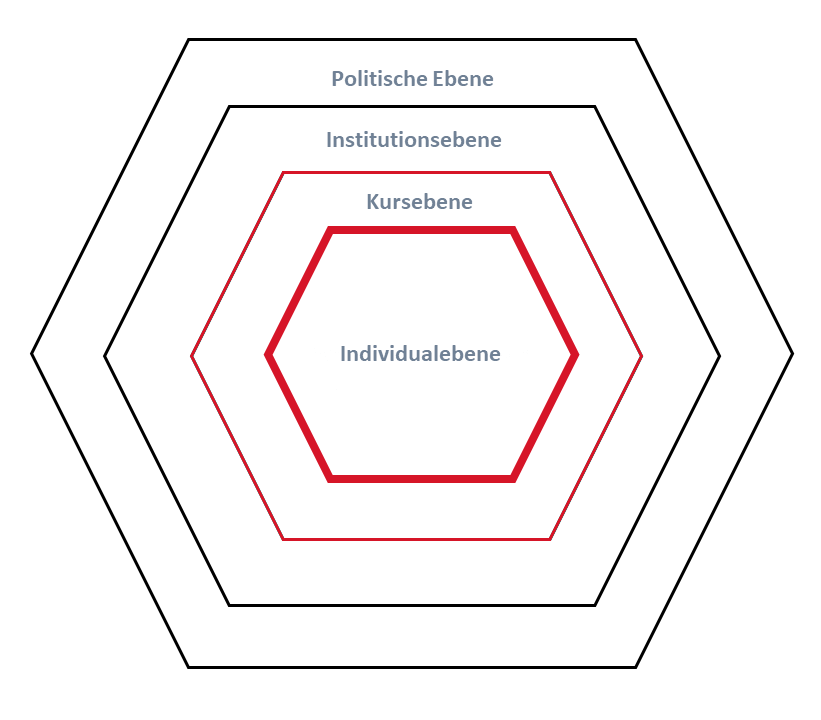
\includegraphics[width=.7\textwidth]{img/Ebenen.png}
        \caption{Aktionsebenen}
        \label{fig:ebenen}
    \end{center}
\end{figure}
%TODO: Verweis auf pptx Fr. Honal % TODO: Gibt es hier noch Quellen?

Durch diesen Fokus entfallen allerdings Vorteile, die sich durch eine größere Nutzer- und damit Datenbasis ergeben.
Besonders die Möglichkeit für Datenanalysen als Teil des Data Minings ist aufgrund des geringen Datenumfangs nicht möglich.
Gleichzeitig sind wir der Überzeugung, dass eine Auswertung des Lernfortschrittes nicht der primäre Grund für die Entwicklung einer Anwendung sein sollte, sondern der Mehrgewinn für Studenten.
Sollte sich die Anwendung für Nutzer als Vorteilhaft erweisen, kann die Anwendung ohne Probleme um Funktionalitäten aus anderen Ebenen erweitert werden.



% TODO: Können Wir vielleicht noch einen User Acceptance Test machen?

% Um eine Fortführung und Integration der anderen Ebenen in Zukunft zu ermöglichen, soll die Datenhaltung und Architektur der Anwendung so konzipiert werden, dass eine Erweiterung leicht möglich ist.

% TODO: Also bauen wir einen Export? Das wäre gut, dann können wir das schreiben. Aber da müssen wir mal schauen. Vordefinierte Auswertungen, Berechnungen wird es allerdings aufgrund der gewählten Abgrenzungen erst einmal nicht geben.
% Die vorhandenen Daten sollen im Ersten Schritt in einem auswertungstauglichen Format zur Verfügung gestellt werden.
% Die Auswertung selbst muss durch den Dozenten selbst erfolgen.

% TODO: Abgrenzung zu anderen Werkzeugen
\subsection{Abgrenzung zu anderen Anwendungen}
Im Hochschulkontext kommen bereits mehrere Systeme zum Einsatz.
Die primäre Plattform bildet \enquote{Moodle}.
Moodle ist eine Lernplattform, in dem Nutzer Kurse, Kalender, Foren und ähnliche Funktionen anbietet, die zur Steuerung und Verwaltung von Vorlesungen bietet.
Trotz des recht umfangreichen Funktionsumfangs besitzt die Anwendung aber einige Nachteile.
So berichten viele Nutzer (Studenten, Dozenten und Unternehmensbetreuer) von sehr schlechter Bedienbarkeit und Unübersichtlichkeit.
Zusätzlich weißt die Datenschutzerklärung darauf hin, dass umfangreich Daten, z.\,B. \enquote{ob und wie sie [Nutzer] in Workshops mitgewirkt haben}, gesammelt werden können.\autocites{moodleTermsOfServiceDHBW}{moodleTermsOfService}
Aus Datenschutzrechtlichen Gründen, wird aktuell die Learning Analytics Erweiterungen und Möglichkeiten der Kursmanagement und Lernplattform Moodle nicht genutzt.

Ein weiteres Werkzeug, welches von im Hochschulkontext verwendet wird ist \enquote{Dualis}.
Diese Anwendung besitzt aber nur Auskunft über Bewertungen.
Anwender können somit erste Feedback zu ihren Klausuren erhalten, sobald sie Klausuren bereits beschrieben haben.
Somit besitzen die Studenen vor der Klausur oft kein Feedback zu der von ihnen geleisteten Arbeit.

Darüber hinaus existieren Anstrengungen weitere Anwendungen umzusetzen, die aber nicht den Prototypstatus verlassen haben.
Ein Beispiel hierfür ist die MyLA-Anwendung.\autocite{mylaGithub}
Für Dozenten gibt es die Möglichkeit, Umfragen zu erstellen und mit ihren Studierenden zu teilen.
Diese haben dadurch die Chance, ihre Meinung zur Vorlesung mitzuteilen, Gelerntes zu verinnerlichen oder auch um Anmerkungen zu gestellten Fragen zu geben.
Die Plattform ermöglicht es dabei, Umfragen als Vorlage zu speichern, sodass diese in unterschiedlichen Kursen verwendet werden können und zeigt die Ergebnisse der Umfragen graphisch an.

% TODO: evasys   Dann kann man sagen, dass mehrer Anwendungen genutzt werden müssen

% TODO: Hier noch einen Satz, alle anderen Anwendungen sind Käse, und dass wir das alles super toll machen


\section{Ist-Analyse} % TODO: Ist es besser die Ist-Analyse mit den funktionalen Anforderungen zusammen zu zeihen? Ich denke schon!
Bevor die eigentliche Entwicklungs starten kann müssen die aktuellen Probleme und Verbesserungspotenziale analysiert werden.

Dozierende haben aktuell wenig Möglichkeiten zu erfahren, wie ihre Vorlesung in verschiedenen Kursen angenommen wird.
Besonders der Lernstand der Studierenden und die Stimmung innerhalb der Kurse sind nur schwer erfassbar.
Nach Aussage eines Dozenten wurde uns gesagt, dass dies besonders in Online-Vorlesungen problematisch ist.
Sofern man \enquote{nicht in fragende Gesichter schaut}, ist es ob schwer zu wissen, wann eine Fragestellung zu kompliziert ist.
Besonders durch die anonyme Maße in Online-Vorlesungen, die auch keine Kameras besitzen dies ein erhebliches Problem.
Dadurch entsteht eine Differenz, die sich in Klausuren negativ auswirken kann.
Aktuell (Dezember '20) finden zum zweiten Mal ausschließlich Online-Vorlesungen statt, sodass diese Möglichkeiten für Dozierende nochmals relevanter sein könnten.



\section{Anforderungsformulierung}

\subsection{Funktionale Anforderungen} 
Bei der Anforderungsanalyse gehen wir nach dem Motto "Von Studenten für Studenten" vor.
Wir als Studenten der DHBW können sehr gut einschätzen was uns das Studium erleichtern würde und wie wir uns in Bezug auf Klausuren und Prüfungen organisieren.
Mit einer Prozessierung und Automatisierung können Synergien genutzt werden und auch andere Kommilitonen von den für diese Veranstaltungen eingebrachten Aufwänden profitieren.

Ziel dieser Arbeit ist es eine App zu entwickeln, die Plattform unabhängig als Web-Applikation oder im Browser genutzt werden kann.
Dabei sollen sowohl Studenten als auch Dozenten einen Zugang bekommen.
Wir setzen auf eine freiwillige Teilnahme.
Die Anwendungen soll durch ihre Funktionen und die intuitive Bedienbarkeit überzeugen und nicht durch einen Nutzungszwang.

Wir konnten die folgenden funktionalen Anforderungen definieren:
\begin{itemize}
    \item Anmeldung                         \\
        Es muss eine Möglichkeit geben, wie neue Studenten und Dozenten die Anwendung nutzen können.
        In der DHBW kommen mit jedem Semester neue Studenten und neue Dozenten.
        Aus diesem Grund muss es eine Möglichkeit geben, neue Nutzer für die Nutzung der Anwendung zu authorisieren.
        Eine Anmeldung kapselt außerdem die Daten einzelner Nutzer.
    \item Kurszuweisung                     \\
        In \autoref{sub:abgrenzung} wurde bereits beschrieben, dass die Kursebene abgedeckt wird.
        Aus diesem Grund muss es eine Möglichkeit geben, Studenten zu Kursen zuzuweisen.
        Kurse sollen dabei eine logische Abgrenzung bilden, sodass Studenten nicht den Lernstoff zwischen verschiedenen Vorlesungen durcheinander bringen.
    \item TODOs                             \\
        Bisher ist es schwer einen Überblick über alle Aufgaben zu haben, die von Studenten zu erledigen sind.
        Besonders die Vielzahl an Vorlesungen, die sich in ihrem Aufbau und in der Prüfungsweise unterscheiden brauchen unterschiedliche Vorbereitungen und damit TODOs.
        TODOs können dabei optional ein Fälligkeitsdatum besitzen, welches zur besseren Organisation sollen die eingetragenen TODOs graphisch angezeigt werden.
        So entsteht ein Kalender und Kapazitätsengpässe rechtzeitig erkannt und durch Umplanen verhindert werden können.

    \item Karteikarten                      \\
        Für eine bessere Prüfungsvorbereitungen Karteikarten angelegt werden.
        Die Karteikarten sollen direkt in App gelernt werden, sodass kein zusätzlicher Aufwand für das Abschreiben der Karten notwendig ist.

    \item Prüfungsterminübersicht           \\
        In der Anwendung soll es eine Übersicht aller Klausuren und anderen Prüfungsleistungen geben.
        Momentan wird dies über einen Google Kalender gehandhabt, welcher über eine Zwischeninstanz verwaltet wird.
        In dem dies direkt in der Anwendung angegeben ist, können zusätzliche Informationen (z.\,B. zugelassene Hilfsmittel) leichter kommuniziert werden und die zeitliche Differenz wird aufgehoben.

    \item Kursübergreifende Informationen   \\
        Besitzt ein Nutzer einen Account, soll er Kurse anlegen können, zu denen er Informationen wie Datum von Prüfungen erfassen kann.
        Um zu verhindern, dass diese organisatorische Aufwand von jedem Studenten einzeln durchgeführt werden müssen soll es zusätzlich die Funktion geben, dass Dozenten einen Kurs anlegen können.
        Den Kursen können initial bereits Prüfungstermine, TODOs und Karteikarten mitgegeben werden.
        Somit entfällt die initiale Erstellung.
        Die zu einem Kurs gehörenden Informationen können von den Studierenden weiterhin nach belieben angepasst und ergänzt werden ohne dabei für die anderen eingeschriebenen Kursteilnehmer Daten zu verändern.
        Das Erstellen eines Kurses hat für den Dozenten den Vorteil, dass für diesen Kurs Daten zur Verfügung gestellt bekommt, die er zur Anpassung oder Evaluation seiner Vorlesung nutzen kann.
        Beispiele hierfür können sein Lerntypen der Studenten, Fortschritt beim Lernen der Karteikarten, etc.
    \item Rollendifferenzierung             \\
        Aus den bereits beschriebenen Anforderungen geht hervor, dass es eine Weise geben muss, wie Dozenten von Studenten unterschieden wird.
        Es soll verhindert werden, dass Studenten falsche Informationen bereitstellen können und so andere Studenten des gleichen Kurses schädigen.
        Aus diesem Grund sollen nur Dozenten Informationen bereitstellen können, die von mehreren Studenten eingesehen werden können.
\end{itemize}

% Das ist das was ich grad realistisch sehe. Wenn wir noch mehr implementiert haben, dann können wir das gerne noch erweitern

% TODO: Wo kommen die Personas hin? vor die Anforderungen? Vielleicht über die Anforderungsanalyse



\subsection{Nicht-Funktionale Anforderungen}
Neben den funktionalen Anforderungen gibt es auch einige nicht-funktionale Anforderungen, die beachtet werden müssen.
\begin{itemize}
    \item Geschwindigkeit\\
        Für Nutzer ist die Geschwindigkeit besonders wichtig.
        Lang ladende Anwendungen sind nicht nur nervig in der Benutzung, sondern könnten sich in der hier entwickelten Anwendung negativ auf den Lernfortschritt auswirken. Lange Ladezeiten lenken beispielsweise ab und demotivieren die Nutzung der Anwendung.
        Über lange Ladezeiten beschweren sich in einer Umfrage mehr als 70\%, wobei 25\% aller Nutzer bereits bei 4 Sekunden die Seite verlassen.\autocite{loadingTimes}
        Aus diesem Grund sollte die Ladezeit gering gehalten werden.
    \item Persistenter Speicher             \\
        Informationen über Kurse müssen dauerhaft gespeichert sein und jederzeit abrufbar sein.
        Besonders vor und nach Vorlesungen wird die Nutzung der Anwendung vorraussichtlich deutlich ansteigen.
        Auch bei Spitzenlast müssen stets alle Informationen abrufbar sein.
    \item Responsive Design\\
        Die Anwendung sollte auf jeden Gerät vollständig funktional sein.
        Studenten nuten häufig viele Geräte mit verschiedenen Bildschirmformaten.
        Besonders unterwegs oder in öffentlichen Verkehrsmitteln sind Mobilgeräte die primären Geräte.
        Aus diesem Grund muss sich die Anwendung dynamisch an solche Geräte anpassen.
    \item Corporate Design\\
        Die DHBW besitzt ein einheitliches Design, an der man alle DHBWs und DHBW-Anwendungen erkennt.
        Damit die Anwendung sich an die DHBW angliedert, sollte die Anwendung nahe an diesem Design sein.
        Besonders das Farbschema sollte dabei einheitlich sein. % TODO: Muss das wirklich sein, das sieht halt echt nicht gut aus. Ich mag das cosmic theme ganz gern
    \item Datenschutz\\
        Das Thema Datenschutz ist so wichtig wie nie zuvor.
        Besonders der Schutz von personenbezogenen Daten steht dabei im Vordergrund.
        Wie oben bereits festgestellt wurde besitzen Anwendungen gegenwärtig problematische Datenschutzlagen.
        Aus diesem Grund soll die entwickelte Anwendung einen hohen Wert auf den Datenschutz legen und die Verarbeitung dieser Daten auf ein Minimum reduzieren.
\end{itemize}



\subsection{Zusammenfassung}
Die gerade beschriebenen funktionalen und nicht-funktionalen Anforderungen sind noch übersichtlich und für die spätere Referenz in \autoref{tab:anforderungen} dargestellt.


\begin{table}[h]
    \centering
    \begin{tabularx}{.8\textwidth}{l|X}
        Nr.     & Beschreibung                              \\\hline
        F1      & Neue Nutzer können sich für die Nutzung anmelden                    \\
        F2      & Studenten können für Kurse eingeschrieben werden  \\
        F3      & Es können TODOs erstellt werden   \\
        F4      & Es kann mit Karteikarten gelernt werden  \\
        F5      & Prüfungstermine können eingetragen werden  \\
        F6      & Informationen können allen Studenten mitgeteilt werden  \\
        F7      & Es gibt eine Unterscheidung zwischen Studenten und Dozenten  \\
        NF1     & Anwendung lädt schnell                    \\
        NF2     & Daten jederzeit einsehbar                 \\
        NF3     & Anwendung funktioniert auf allen Geräten  \\
        NF4     & Anwendung ist am DHBW Design orientiert   \\
        NF5     & Personenbezogene Daten werden geschützt  \\
    \end{tabularx}
    \caption{Zusammengefasste Anforderungen}
    \label{tab:anforderungen}
\end{table}

% TODO: Wenn das Dashboard fertig ist, stehen da ja dann Analysen drin? Dann kann man das alles noch erweitern
% Generell Umfragen, .... alles erst reinschreiben, wenn wir das auch implementiert haben :)


% !TEX root =  ../master.tex
\chapter{Konzeption}
Bevor mit der Implementierung gestartet werden kann wird ein Konzept erstellt, welches als Leitfaden für die Implementierung dienen soll.
Ziel ist ein konkreter Entwurf, welcher die technischen und grundlegenden Funktionalitäten beschreibt.
Dadurch soll verhindert werden, dass die aufwendige Implementierung fehlschlägt oder mehrfach Änderungen durchgeführt werden müssen, welche den Implementierungsaufwand vergrößern würden.


















\section{Konzeption der Anwendungsarchitektur}
Die Grundlage jeder Anwendung ist der Aufbau und die Struktur der Infrastruktur, auf welcher die Anwendung später ausgeführt werden soll.
Aus diesem Grund wird diese als Erstes betrachtet.

\subsection{Traditionelle Architektur}

Webanwendungen werden üblicherweise in einem Client-Server-Modell entwickelt. Im Konkreten kann hier von einer Thin-Client Architektur gesprochen werden, da jegliche Anwendungsdatenverarbeitung Server-seitig durchgeführt wird \autocite{definitionOfThinClient}. % TODO: \autocite{Leff} --> ?
Der Client übernimmt dabei sämtliche Funktionalitäten, die das Nutzerinterface betreffen. Über diese Aufteilung von Verantwortlichkeiten können Wartung und Sicherheit durch die zentrale serverseitige Verwaltung in einem Rechenzentrum einfacher gesichert werden. Falls der Client selbst Daten verarbeiten und speichern würde, könnte dies zu inkonsistenten Daten und Sicherheitslücken führen, da unterschiedliche Datenbestände zwischen Client und Server entstehen könnten. 
Visualisierung und die Interaktion mit dem Nutzer fallen hierbei in die Aspekte des Nutzerinterfaces, worüber diesem die Interaktion mit den zentralen Datenbeständen ermöglicht wird. Dabei wird jedoch keine Anwendungslogik ausgeführt \autocite{thinClientArchitectureOverview}. Es ist allerdings wichtig zu betonen, dass diese Nutzerschnittstelle essentiell für den Erfolg der Anwendung ist. Eine maximale User Experience \autocite{definitionUserExperience} zu bieten ist ein kritischer Faktor für die Qualität der Nutzerschnittstelle \autocite{thinClientArchitectureOverview}.\\
Entsprechend wird die gesamte Geschäftslogik, Datenhaltung und der Datenaustausch von einem zentralen Server verwaltet. 
In \autoref{fig:clientServerAufbau} ist eine solche Architektur vereinfacht dargestellt, wobei zwischen dem Anwendungs- und dem Datenbankserver unterschieden ist. Der Anwendungsserver beinhaltet hierbei sämtliche Geschäftslogik- und Datenaustauschzuständigkeiten. Der Datenbankserver ist hingegen ausschließlich für die persistente Datenhaltung zuständig.

\begin{figure}[h]
    \centering
    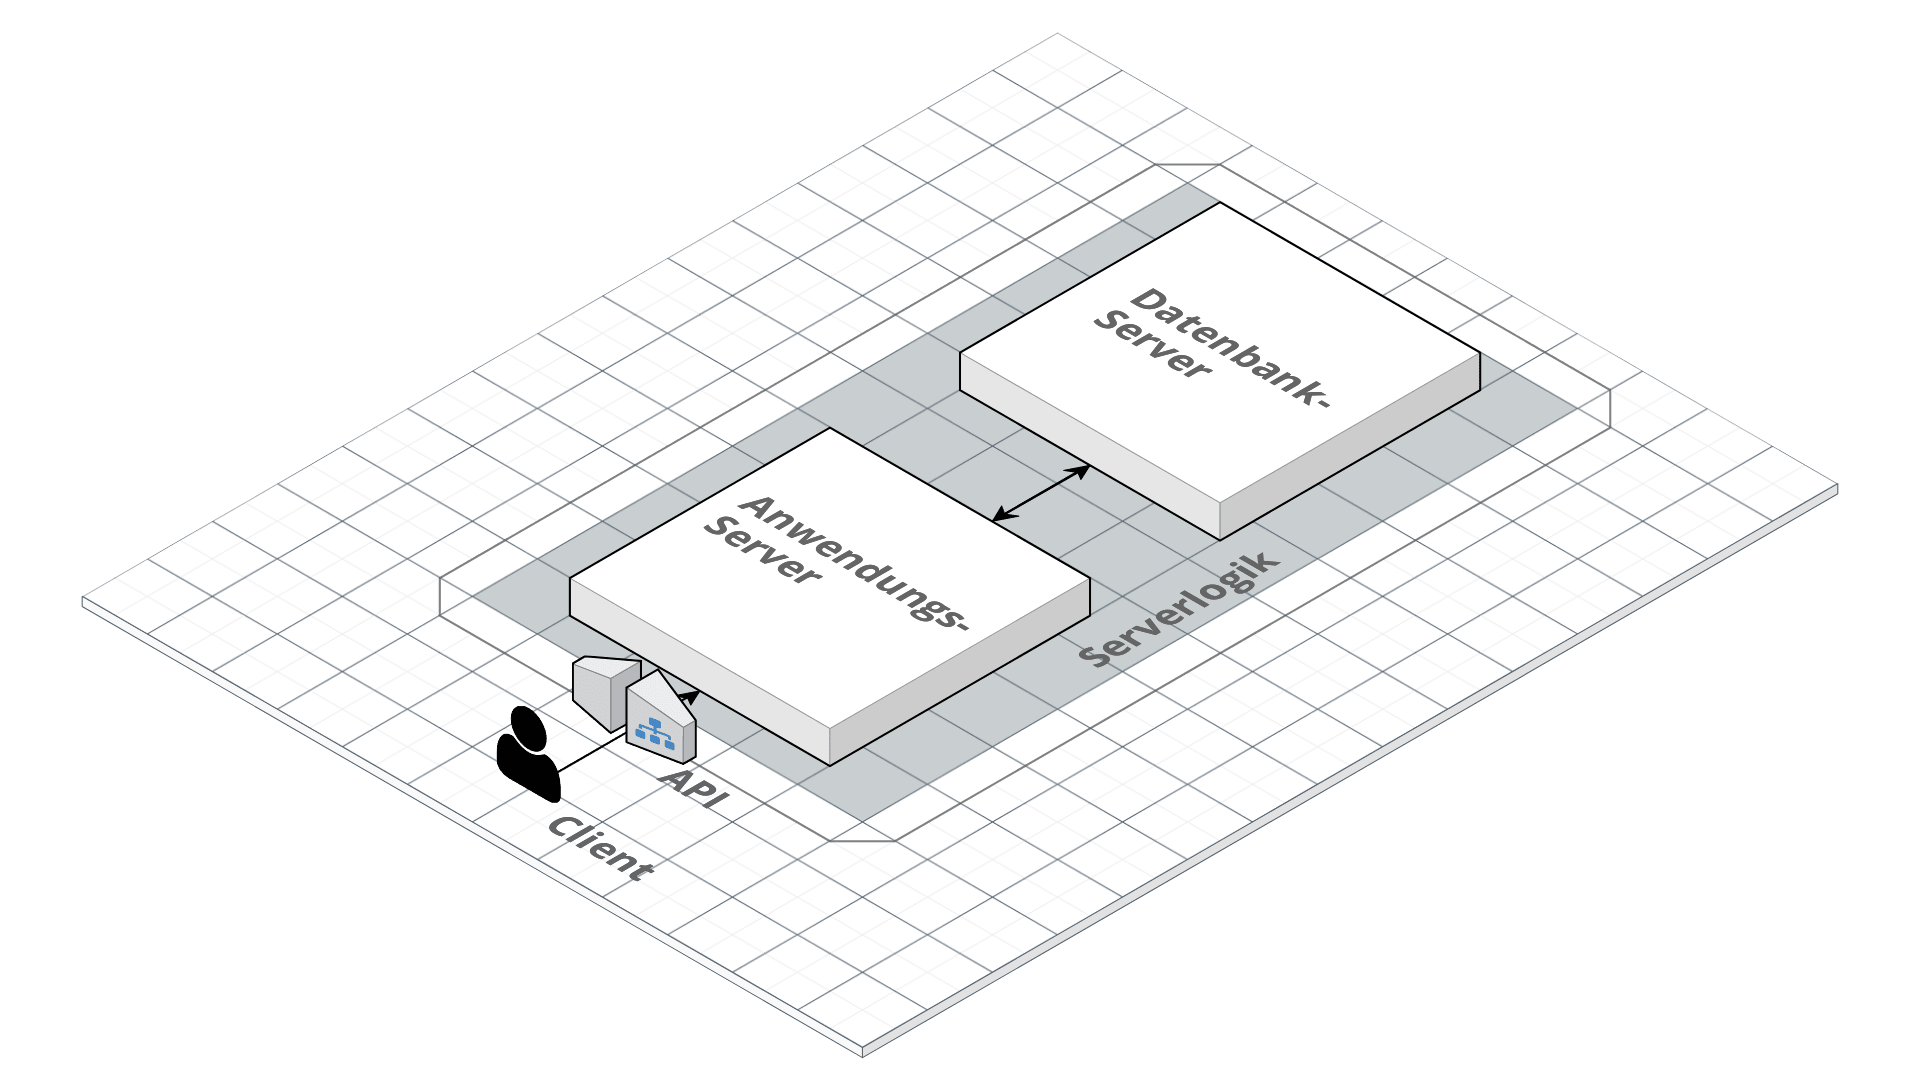
\includegraphics[width=.9\textwidth]{img/ClientServer.png}
    \caption{Vereinfachter Client-Server-Aufbau}
    \label{fig:clientServerAufbau}
\end{figure}

Praktisch dargestellt, ruft der Nutzer mithilfe seines Browsers die Webseite von einem Server ab.
Der Browser verarbeitet mithilfe der implementierten Geschäftslogik die Anfrage des Nutzers und greift auf die Daten des Datenbankservers zu. Diese Daten werden schließlich dem Nutzer zur Verfügung gestellt, welche ihm in der Nutzerschnittstelle angezeigt werden und für ihn an  dieser Stelle aufbereitet einsehbar sind.\\
Dabei greift der Nutzer über ein wohldefiniertes \ac{API} auf den Anwendungsserver zu, um diesen dargestellten Prozess abzusichern.

%Dieser läd die notwendigen Informationen auf ähnliche Weise von einem Datenbankserver und bereitet diese gegebenenfalls auf. edit pdm: im Absatz obendrüber bearbeitet
%Der Nachteil von Client-Server-Modellen ist der hohe Aufwand im Bereich der Skalierung. edit pdm: im Absatz untendrunter bearbeitet

Nach den Anwendungsanforderungen wird eine hohe Leistungsfähigkeit benötigt, die auch mit Leistungsspitzen klar kommen muss. Da anzunehmen ist, dass der Großteil der Nutzer in der Mitteleuropäischen Zeitzone vorzufinden sein wird, können solche Leistungsspitzen morgen zu Vorlesungsbeginn, nach der Mittagspause oder am frühen Abend auftreten. Bei diesen Leistungsspitzen ist eine hohe Serverkapazität notwendig.
Hierbei müssen sowohl die implementierte Serverlogik, als auch die zugrundeliegende Serverinfrastruktur konsistente Daten mit akzeptablen Antwortzeiten liefern. Diese Vorgänge fallen in den Bereich der Skalierung, welcher sowohl für die Serverlogik, als auch für Infrastruktur einen hohen Aufwand birgt.\\
Um dieses Problem zu lösen gibt es zwei Lösungsansätze. In der ersten Lösung können permanent Serverressourcen bereitgestellt werden, die auch bei Leistungsspitzen nicht überlastet sind und ausfallen, jedoch würden bei dieser Lösung viele Ressourcen in \enquote{Ruhephasen} ungenutzt bleiben, was unökonomisch und kostspielig wäre.\\
In der zweiten Lösung können notwendige Serverressourcen an Leistungsspitzen dynamisch hinzugezogen werden. Hierbei besteht jedoch die Schwierigkeit, diese Leistungsspitzen rechtzeitig zu erkennen, um frühzeitig Serverressourcen steigern zu können. Sofern diese Schwierigkeiten bei dem zweiten Lösungsansatz umgesetzt werden können, ist dies eine optimale Lösung, jedoch ohne weiteres nicht einfach umzusetzen.\\






\subsection{Serverless Architektur}
Serverless-Architektur ist ein relativ neuer Ansatz, mit dem die Entwicklung von Web- und Mobilanwendungen beschleunigt werden soll.
Hierbei steht die Nutzung von CLoud-Providern im Vordergrund, die sich um die notwendige Server-Architektur kümmern. Entwickler müssen lediglich die Anwendungslogik in der Cloud (zum Beispiel in Form einer Funktion) erstellen, ohne diese auf einem dezidierten Server bereitzustellen.
Hierbei können je nach Nutzeranforderungen Ressourcen bereitgestellt und auch wieder entzogen werden. Der Entwickler einer Anwendung muss nur die verwendeten Ressourcen (somit Netzwerkverkehr, Prozessorrechenzeit und generelle Verarbeitungszeit) bezahlen. Ressourcen können hiermit dynamisch bei Leistungsspitzen in großem Umfang zur Verfügung stehen.

Dieses Serverless Computing kann in \ac{BaaS} und \ac{FaaS} unterteilt werden \autocite{whatIsServerless}. Hierbei ist zu unterscheiden, dass bei \ac{BaaS} dem Entwickler weitere Backend-Funktionalitäten zur Verfügung gestellt werden, welche er in seiner Anwendungs- (und damit Geschäfts-)logik verwenden kann, womit die Skalierbarkeit der entwickelten Lösung nochmals an vielen Stellen verbessert werden kann. Aus diesem Grund haben wir uns für einen solchen \enquote{Serverless}-Ansatz entschieden.

\ac{BaaS} ist ein relativ neuer Ansatz, mit dem die Entwicklung von Web- und Mobilanwendungen beschleunigt werden soll.
Bei \ac{BaaS} handelt es sich um ein Cloud-Service-Modell, welches sich aus der steigenden Nutzung von Cloud-Computing und Serverless-Ansätzen ableitet.
Dabei geht \ac{BaaS} einen Schritt weiter als andere Cloud-Ansätze wie \ac{IaaS}, \ac{CaaS} oder \ac{FaaS}.
Stattdessen orientiert sich \ac{BaaS} mehr an einem \ac{SaaS}-Ansatz. % :D xD O: (:
So wird in \ac{BaaS} nicht nur die gesamte Infrastruktur und Laufzeitumgebung, sondern sogar Teile der Serverlogik von einem Cloud-Provider verwaltet\autocite[Vgl.][]{cloudflareBaaS} und Anwendungsentwickler können sich auf die Entwicklung der Nutzeranwendungen und die Geschäftslogik kümmern, ohne umfangreichen Boiler-Plate-Code schreiben zu müssen.
Typische Beispiele für Services, die von einem \ac{BaaS}-Anbieter übernommen werden, sind die Bereitstellung von Speicherressourcen, Nutzerauthentifizierung und das Hosting einer Website.
Diese Themenbereiche sind Services, die in fast jeder Anwendung benötigt werden, wodurch ein großer Teil der Entwicklung eingespart werden kann.
Dadurch spart es Kosten in Form von Serverequipment, Know-How und Entwicklungsressourcen.

\begin{figure}[h]
    \centering
    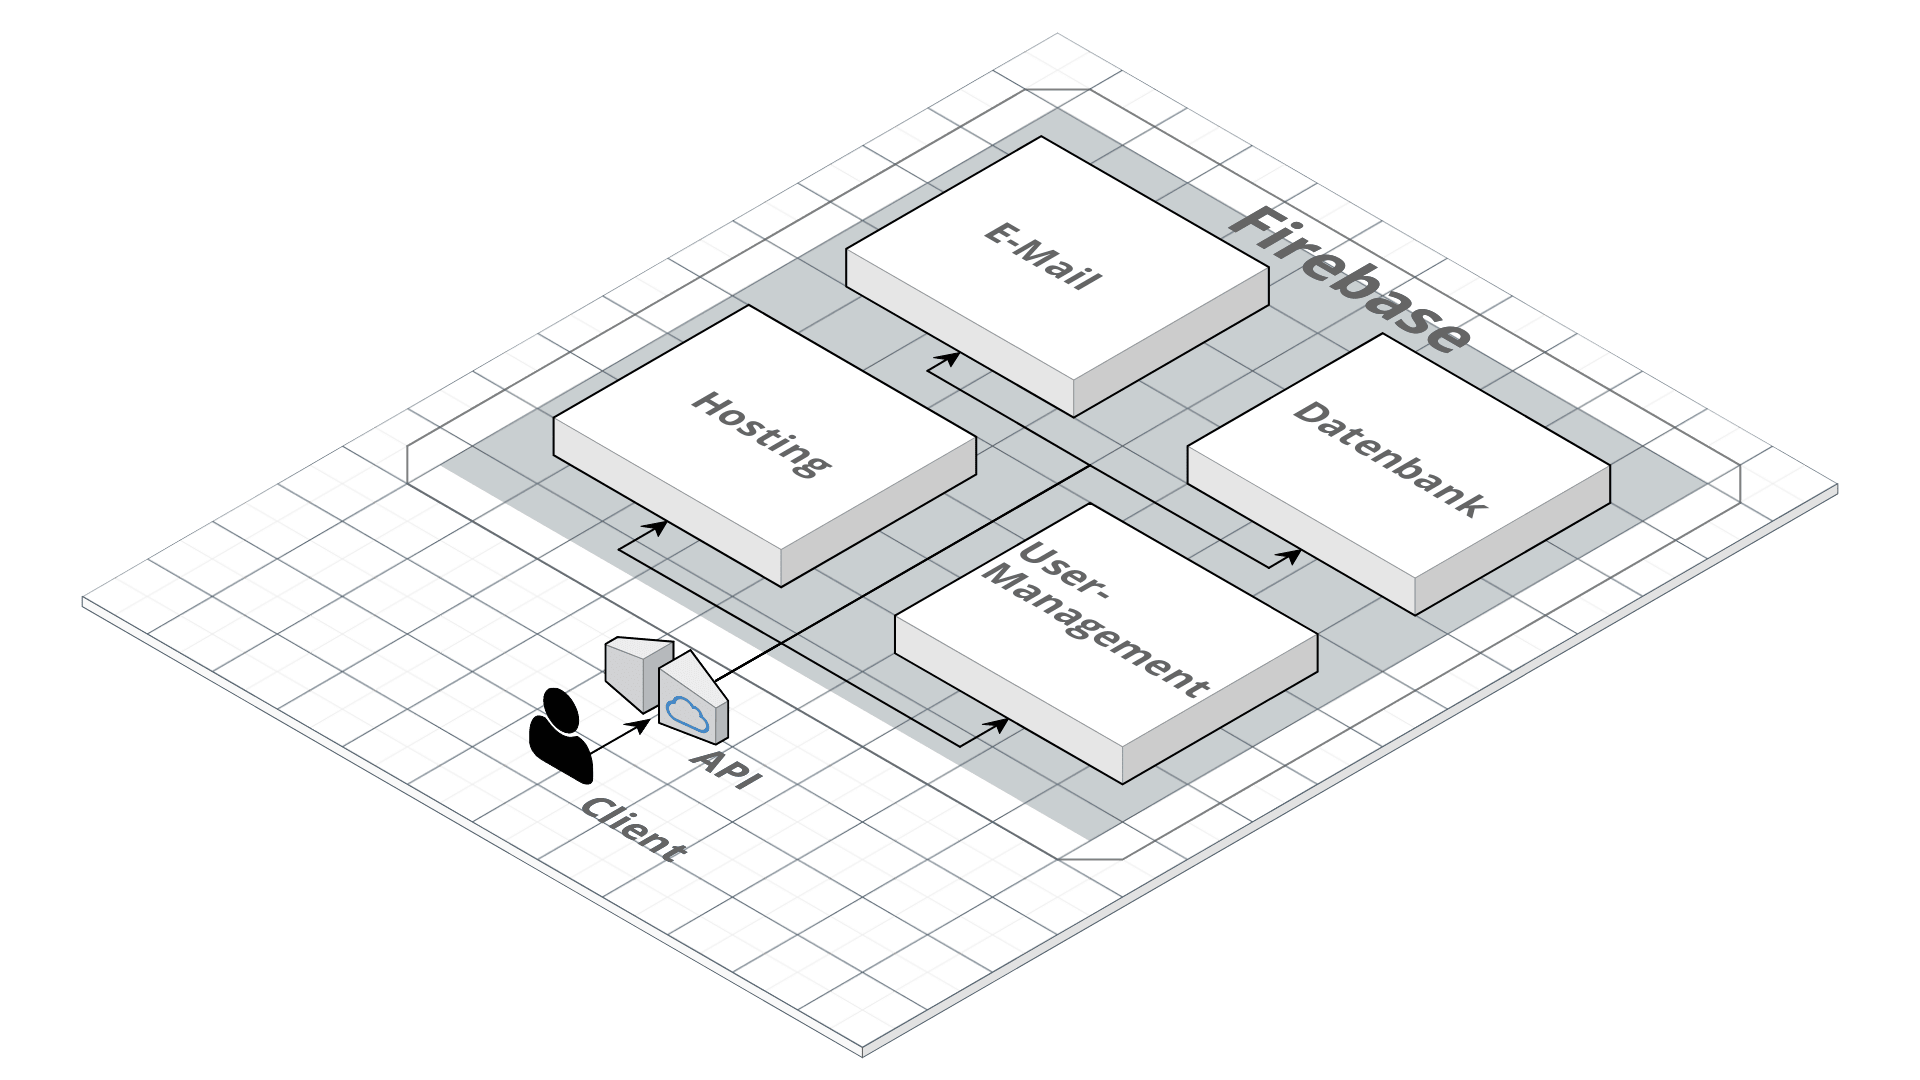
\includegraphics[width=.9\textwidth]{img/Firebase.png}
    \caption{Vereinfachter Firebase-Aufbau}
    \label{fig:firebaseAufbau}
\end{figure}


Wir haben uns für die Verwendung von Firebase als eine solche Lösung entschieden.
Firebase ist ein \ac{BaaS}-Dienst von Google LLC.
Firebase wurde aus einer Reihe von Gründen für die Entwicklung der Anwendung ausgewählt:
\begin{itemize}
    \item Datensicherheit\\
        Nach einer Befragung von Tang und Liu stimmen 48\% zu, dass Cloud-Provider eine bessere Sicherheit liefern als eigene Implementierungen.\autocite[S. 63]{TANG}
        Google als einer der größten IT-Dienstleister ist dabei weit vorne und ist konform mit den europäischen Datenschutzverordnungen.\autocite{firebaseDataprotection}
        Die Authentifizierung ist sicher, da aktuelle Standards wie OAuth 2.0 verwendet werden.
    \item Ausfallsicherheit\\
        Da Server nicht mehr einzeln betrieben werden müssen entfällt die Gefahr eines \enquote{Single Point of Failure}. %TODO: in die Anforderungen
        Dieser wäre dafür verantwortlich, dass die Anwendung ausfällt, sofern der Server abstürzen würde.
        Firebase und Google bieten stattdessen ein \ac{SLA} an, das eine Ausfallsicherheit von mehr als 99,9\% garantiert.\autocite{firebaseSLA}
    \item Komplexität\\
        Da Entwickler nun nur noch das Frontend entwickeln müssen und sich nicht mehr um das Backend oder die Kommunikation zwischen den Komponenten kümmern müssen, wird die Entwicklung vereinfacht und beschleunigt.
        Die Entwicklung des Frontends kann vorranschreiten, ohne auf die Entwicklung des Backends warten zu müssen.
    \item Kosten \\
        Google bietet attraktive Preismodelle an, welche die Bereitstellung der Anwendung sehr kostengünstig machen.
        Nicht nur entfallen Kosten für die Wartung der Server und Hardwareressourcen, sondern der gesamte Betrieb ist im \enquote{Spark}-Plan kostenlos.
    \item Skalierung \\
        Firebase kümmert sich um die gesamte Bereitstellung und Skalierung der Serverleistung.
        Das heißt, sofern mehr Rechenleistung benötigt wird (wie beispielsweise in Lastspitzen), wird die Rechenleistung automatisch erhöht ohne so das fehlschlagen von Anfragen vermieden.
\end{itemize}




















\section{Konzeption der Funktionalitäten}\label{sec:konzeptionFunktionalitaeten}


\subsection{Kurse}

Informationen sollen in Kurse unterteilt werden.
Aus diesem Grund wird eine Möglichkeit benötigt, wie Nutzer Kurse wechseln können und erkennen können zu welchem Kurs die Informationen gehören.
Auch hier gibt es mehrere Möglichkeiten, wie eine solche \ac{UX} gestaltet werden kann, die jeweils verschiedenen Vor- und Nachteilen besitzen.

Eine Möglichkeit ist die gesamte Anwendung innerhalb eines Kurses anzubieten.
Das heißt, der Nutzer hat nach dem Login die Möglichkeit einen seiner Kurse auszuwählen.
Dieser Kurs wird anschließend geladen und der Nutzer sieht nur die Informationen dieses Kurses.
Möchte man den Kurs wechseln, gibt es ein Bento-Menü, über welches ein anderer Kurs ausgewählt werden kann.
Eine solche \ac{UX} hat den Vorteil, dass sich ein Nutzer vollständig auf einen Kurs konzentrieren kann und so nicht Informationen zwischen verschiedenen Kursen durcheinander wirft.
Gleichzeitig kann dies aber dazu führen, dass ein Nutzer eventuell den Überblick über seine Kurse verliert und so einen Kurs womöglich vernachlässigt.
Auch Kursübergreifende Informationen, z.\,B. TODOs, können nur schwer abgebildet werden, ohne das die Nutzung der Anwendung erklärungsbedürftig wird.

Als zweite Möglichkeit kommt eine virtuelle Trennung zum Einsatz.
Dabei sieht der Nutzer alle Informationen und eine Trennung dieser findet nur über die Navigation statt.
So besitzt die Anwendung für jeden Kurs einen eigene Sektion, in der die Informationen dargestellt werden.
Dadurch kann der Nutzer stets alle Kurse sehen und die \ac{UX} wird vereinfacht.



\subsection{Rollenzuweisung}

Aus den Anforderungen geht hervor, dass es zwei Nutzerrollen gibt: Dozenten und Studenten.
Dozenten sollen in der Anwendung ihre Kurse verwalten können.
Ein Kurs orientiert sich dabei an der Organisation, die in der Realität vorliegen.
Auch in vorhandenen Tools wie beispielsweise \enquote{Moodle} sind Studenten anhand von Kursen organisiert.
Aufgrund der Vielzahl an solchen Lösungen scheint sich eine solche Organisation zu bewähren.
Aus diesem Grund liegt es nahe, das auch die zu entwickelnde Anwendung eine solche Struktur nutzen sollte.
% TODO: Wie Werden Kurse erstellt

Nachdem nun geklärt wurde, wie die Organisation von Studenten und Dozenten stattfindet, muss nun die Zuweisung von Studenten zu Kursen die Zuweisung von Dozenten konzipiert werden.
Zunächst wird die Studentenzuweisung betrachtet.
Für die Zuweisung von Studenten kommen mehrere Ansätze in betracht, die sich in der Person unterscheiden, die die Zuweisung durchführt:
\begin{enumerate}
    \item Zuweisung durch Anwendungsadministrator
    \item Zuweisung durch Dozenten
    \item Zuweisung durch Studenten
\end{enumerate}
Als erster Ansatz kommt die Zuweisung durch einen Anwendungsadministrator in betracht.
Ein solcher Administrator ist ein zentraler Mitarbeiter der DHBW, welcher komplette Autorität über die Anwendung besitzt.
Von einem solchen Ansatz wird abgesehen, da der Verwaltungsaufwand sehr hoch ausfällt.
Für jeden Kurs über 20 Studenten zuzuweisen, und das für mehrere Kurse pro Semester und Vorlesung, scheint nicht realistisch.

Der zweite ist der Ansatz der Zuweisung durch einen Dozenten.
In der aktuellen DHBW-Organisation besitzen Dozenten bereits eine Liste an Studenten für ihre Vorlesung.
Diese Liste dient zur Anwesendheitskontrolle.
Demnach können Dozenten diese Liste für die Zuweisung in der Anwendung nutzen.
Der Nachteil eines solchen Ansatzes ist es aber, dass Studenten ihre Daten in der Anwendung hinterlassen müssen und diese durch andere Dozenten gegebenenfalls einsehbar wären.
Zusätzlich geht die Anonymität, welche durch Matrikelnummern gegeben ist eventuell verloren.
Insgesamt ist dieser Ansatz aus Datenschutzaspekten besonders kritisch. % TODO: Beim Admin nicht so, weil dhbw

Als Letzter Ansatz ist die Zuweisung durch den Studenten.
Denkbar sind hier mehrere Ansätze: Eine Liste aus Kursen oder über einen Kursidentifikator.
Eine Liste mit Kursen vereinfacht die Zuweisung durch den Studenten, da Kurse schnell entdeckt werden können und eventuell zusätzliches Wissen vermittelt werden kann, wenn der Student sich für mehrere ähnliche Kurse einträgt.
Nachteil ist aber die unmittelbare Verwaltung und Übersicht über die Kurse.
Eine Zuweisung über einen Kursidentifikator (kurz: Schlüssel) hat den Nachteil, dass diese Schlüssel erst aufwändig über einen weiteren Kommunikationsweg (z.\,B. Email oder direkt in einer Vorlesung) mitgeteilt werden muss.
Dafür besitzen Studenten aber nur Zugriff auf die für sie relevanten Vorlesungen.
In \enquote{Moodle} ist die Zuweisung zu Kursen auf freiwilliger Basis anhand von Einschreibeschlüsseln gelöst.
Aus diesem Grund ist dieser \enquote{Workflow} bereits für Studenten bekannt und eine Anpassung an die neue Anwendung ist schnell möglich.
In der Tat nutzen viele existierende Anwendungen ein solches System.
Beispiele hierfür sind Zoom oder Google Meets.


\subsection{Registrierung}
Nutzer der Anwendung können sich selbst registrieren.
Daraus ergibt sich die eine Rollen Problematik: Woran kann die Anwendung erkennen, welcher Nutzer ein Student ist und welcher Nutzer ein Dozent ist.
Sofern Nutzer dies selber angeben können, bräuchte es gegebenenfalls eine Validierung durch die DHBW, wodurch erneut die oben genannten Nachteile einer Zuweisung durch einen Administrator greifen.
Ein Ansatz, bei dem Nutzer dies selber verwalten können wird auch hier als besser angesehen.
Aus diesem Grund wird der folgende Ansatz verwendet:
Statt festdefinierte Rollen (Student und Dozent) zu besitzen, kann jeder Student selbst sowohl Student, als auch Dozent sein.

Jeder Nutzer ist zunächst keiner Rolle zugeordnet.
Jeder Nutzer kann einen Kurs erstellen, wodurch dieser Nutzer automatisch zu einem Dozent für diesen Kurse.
Sobald sich ein Nutzer mithilfe des Einschreibeschlüssels für einen Kurs anmeldet wird der Nutzer automatisch für diesen Kurs zu einem Studenten.
Dadurch können auch zuvor nicht vorgesehene Nutzerbeziehungen entstehen.
Beispielsweise kann ein Dozent sich in einen weiteren Kurs einschreiben, falls er sich in einer weiteren Richtung weiterbilden möchte.
Oder die DHBW kann sich in für einen Kurs einschreiben um die Qualität einer Vorlesung zu validieren.


Ein Vorteil eines solchen Ansatzes ist es, dass auch Studenten Kurse erstellen können und so Lerngruppen gefördert werden.
Denkbar ist beispielsweise ein Student, welcher Nachhilfe anbietet.
Dadurch wird die Nutzung der Anwendung gefördert.








\subsection{TODOs}
Aus den Anforderungen geht hervor, dass TODOs gespeichert werden sollen. In Einklang mit den anderen Konzeptionen können auch die TODOs an Kurse gebunden werden. Stattdessen haben wir uns dafür entschieden die TODOs zentral und Kursübergreifend zu gestalten. So hat der Nutzer stets Übersicht über alle Aufgaben und es geraten keine Informationen in den Hintergrund.

Neue TODOs sollen einfach hinzugefügt werden können. Aus diesem Grund soll es nur notwendig sein den Namen einer Aufgabe zu definieren und alle anderen Attribute wie Fälligkeitsdaten optional zu gestalten.

Gleichzeitig sollen alle TODOs grafisch dargestellt werden, um die Planung zu erleichtern.
Opimalerweiße sollten die Termine in einem Kalender dargestellt werden.
Je voller ein Tag ist, desto deutlicher soll der Backlog hervorgehoben werden, mit rot als Signalfarbe. Der Kalender soll prominent dargestellt werden, sodass der Nutzer sich sofort einen Überblick verschaffen kann. 


\subsection{Karteikarten}
In den Anforderungen wurde definiert, dass die Anwendung Karteikarten zur Untersützung von Lerninhalten unterstützen soll.
Für das Lernen mit den Karteikarten gibt es eine Vielzahl an unterschiedlichen Algorithmen. Unsere Anwendung soll einen Algorithmus aus dem Bereich der \enquote{Spaced Repetition Systems} implementieren. In die deutsche Sprache übersetzt heißt das so viel wie "Wiederholen ohne Lücken". Das System hinter diesen Algorithmen besteht darin, die entsprechenden Informationen genau dann zu wiederholen, wenn das menschliche Gehirn sie fast schon vergessen hätte.\autocite[Vgl.][]{Tabibian3988} Die einzelnen Karteikarten werden nacheinander abgefragt und bei richtiger Antwort in zunehmenden Zeitintervallen immer wieder überprüft. Durch diesen Abstandseffekt soll gezielt das Langzeitgedächnis trainiert werden, damit die Inhalte auch über eine Prüfung hinaus im Gedächtnis behalten werden. Die unterschiedlichen Algorithmen dieser Klasse unterscheiden sich lediglich in der Wahl der Zeitabstände. 
Genutzt werden soll das Super-Memo System des polnischen Neurobiologen Piotr Wozniak. Es definiert folgende Zeitabstände:
\begin{itemize}
	\item 20 Minuten
	\item 24 Stunden
	\item 48 Stunden
	\item 10 Tagen
	\item 30 Tagen
	\item 60 Tagen
\end{itemize}  
Kann eine Frage nicht beantwortet werden, so wird diese direkt wiederholt und durchläuft die definierten Zeitintervalle von vorn. \autocite[Vgl.][]{BaileyuDavey}



\subsection{Lernmaterialien}
Um das Lernen zu unterstüzen sollen

\subsection{Dashboard}
//TODO

\subsection{Auswertungen}
//TODO




























\section{Datenstruktur}
Aus den in \autoref{sec:konzeptionFunktionalitaeten} entworfenen Funktionalitäten lässt sich ein Entwurf für die Datenhaltung erstellen.

Die Datenspeicherung findet vollständig innerhalb von Firebase statt.
Der hierfür genutzte Service heißt \enquote{Firestore}.
Dabei werden Daten nicht wie in einer klassischen relationalen Datenbank (\ac{RDB}) in Tabellen mit Spalten und Zeilen gespeichert, sondern in Collections aus Dokumenten. Dies erlaubt eine größere Flexibilität in der Entwicklung.


In \autoref{fig:erDiagramm} ist das zugrundeliegende Datenmodell abgebildet, welches in der Implementierung verwendet wird.

\begin{figure}[ht!] % TODO: Hier fehlen die streaks 
    \begin{center}
        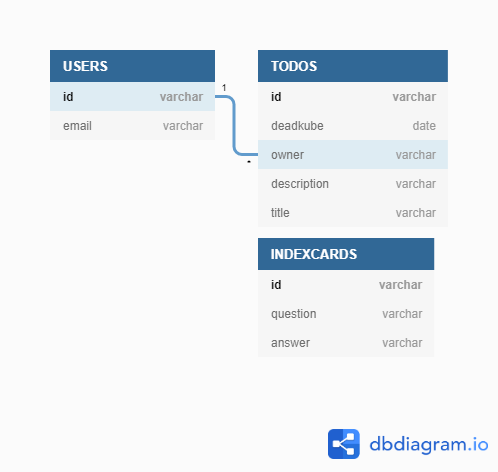
\includegraphics[width=\textwidth]{img/Integrationsseminar ER.png}
        \caption{ER-Diagramm}
        \label{fig:erDiagramm}
    \end{center}
\end{figure}






% !TEX root =  ../master.tex
\chapter{Implementierung}

In \autoref{cha:konzeption} wurde bereits ein Konzept für die Implementierung erstellt. In der Implementierung wurden die Anforderungen wie konzipiert umgesetzt.
Dennoch gibt es einige nicht-funktionale Anforderungen und allgemeine Implementierungsdetails, die noch nicht angesprochen wurden. In diesem Kapitel werden diese genauer beleuchtet.

\section{Dateistruktur}

Auf der obersten Ebene befinden sich alle Dateien, die allgemeine Konfigurationen enthalten. Beispielsweise liegen dort die Firebase-Konfigurationen, die Angular-Konfigurationen und 
weitere technische Konfigurationsdateien. Des Weiteren sind die folgenden zwei Ordner relevant: \enquote{src} und \enquote{docs}. Im docs-Ordner ist die Dokumentation im \LaTeX-Format 
und im src-Ordner ist der gesamte Code enthalten. \\
Im src-Ordner ist nochmal eine weitere Unterteilung in \enquote{assets}, \enquote{environments} und \enquote{app}. Im assets-Ordner sind alle Icons, Designs und Übersetzungen und im environments-Ordner 
liegen die Dateien mit den Daten, welche für das Bauen der Applikation notwendig sind. Im app-Ordner sind zwei wichtige Ordner enthalten, zum einen den auth-Ordner, der den gesamten Code rund um das 
Thema Authentifizierung enthält und dem pages-Ordner, der den restlichen Code für alle Seiten auf der Learning Analytics App enthält. \\

\section{Responsive Design} 
Nach den nicht-funktionalen Anforderungen ist ein responsive Design pflicht.  
Bei der Entwicklung wurde auf die responsive Darstellung geachtet.
So verhalten sich alle Funktionalitäten einer Anwendung wie es von einer nativen Anwendung erwartet wird.
Dies macht sich besonders in der optimierten Darstellung bemerkbar, bei der der Nutzer nicht zu scrollen oder zoomen verpflichtet ist.
Aber auch andere Funktionalitäten, wie das Wischen der Karteikarten, funktioniert auf Geräten mit einem Touchscreen genauso wie auf Geräten, welche eine Maus verwenden.

\section{Zugangskontrolle}
Nach den Anforderungen müssen zwei Rollen unterschieden werden: Studenten und Dozenten.
Die Zugangskontrolle findet an mehrere Komponenten statt: Eine Zugangskontrolle auf Serverseite und eine Navigationskontrolle innerhalb des Nutzerinterfaces.


\subsubsection*{Serverside}
Eine Server-seitige Zugangskontrolle ist notwendig, da Nutzer das Nutzerinterface und den Netzwerkverkehr manipulieren und so Zugang bekommen könnten.
Aus diesem Grund werden sämtliche Serveranfragen validiert.
Dafür sind auf dem Server Regeln hinterlegt, die die Authorisierung des Nutzers überprüfen.
Die Regeln werden bei jeder Anfrage vor der Bearbeitung dieser überprüft.

\begin{lstlisting}[caption={Einfaches Beispiel der Serverside Regeln}, label=lst:firestoreRules]
rules_version = '2';
service cloud.firestore {
    match /databases/{database}/documents {
        function getRole(role) {
            return get(/databases/$(database)/documents/users/$(request.auth.uid)).data.roles[role]
        }
        match /{document=**} {
            allow read:  if request.auth != null;
            allow write: if getRole('dozent')
        }
    }
}\end{lstlisting}


\subsubsection*{Userside}
Auf der Nutzerseite existiert eine Zugangskontrolle, die verhindert, dass ein Nutzer Interfacezustände hervorrufen kann, für die er nicht authorisiert ist.
Ein Beispiel hierfür ist die Navigation auf eine Maske, für deren Daten er Server-seitig nicht berechtigt ist.
In diesem Fall würde der Nutzer Fehlermeldungen und eine schlechte User Experience erleben.
Im Nutzerinterface ist dafür ein \enquote{Router-Guard} implementiert.
Dieser Guard überprüft bei jedem Navigationsversuch, ob der Nutzer für die Zielroute berechtigt ist.
Nur wenn der Nutzer die notwendigen Berechtigungen besitzt, wird die Navigation fortgesetzt.
Nutzer ohne die notwendigen Berechtigungen werden automatisch auf das Dashboard bzw. die Login-Maske geleitet.


\section{Übersetzung}

An der DHBW studieren viele Studenten aus unterschiedlichen Ländern.
Nicht immer ist Deutsch die Muttersprache.
Besonders für Studenten des rasmus+ Programms ist Englisch oft präferiert.

Aus diesem Grund ist die Anwendung sowohl in Deutsch, als auch in Englisch verfügbar.
Neue Sprachen können einfach mithilfe von JSON-Dateien hinzugefügt werden.
Diese JSON-Dateien enthalten alle HTML-Labels und die Übersetzung in die jeweilige Sprache. 
Verfügbare Sprachen werden in der Navigation im Globus-Menue angezeigt.
Durch Klick auf eine Sprache wird sofort die gesamte Anwendung übersetzt, ohne das neu geladen werden muss.
Dabei wird einfach die jeweilige JSON-Datei mit den Labels in der richitgen Sprache verwendet.

Die Anwendung fragt beim initialen Aufruf der Anwendung ab, auf welche Sprache das Gerät des Nutzers eingestellt ist.
Wird eine kompatible Sprache gefunden, so wird die Anwendung in diese übersetzt.
Andernfalls wird Englisch als internationale Sprache gewählt.

Wurde die Registrierung erfolgreich abgeschlossen, wird der Nutzer auf eine freiwillige Umfrage geleitet.
Der Nutzer kann dabei angeben, welcher Lerntyp er ist, wie affin er für die Nutzung von online-Lernplattformen ist und welche Erfahrung er mit diesen bisher gemacht hat.
Leiter von Kursen, in denen dieser Nutzer eingeschrieben ist, können anschließend diese Informationen anonym einsehen.
Dabei existiert ein separater Abschnitt im Feedback, welcher einen Einblick über alle Studenten gibt.
Dies erlaubt es Kursbesitzern bzw. Dozenten, ihren Lerninhalt besser auf die Studenten abzustimmen und die Kursqualität zu erhöhen.
Nutzer können jederzeit über das Profil-Kontextmenü ihre Angaben ändern.

Aufgaben können sowohl ein Start-, als auch ein Enddatum haben.
Existiert nur eines dieser Daten, wird das andere auf den gleichen Tag terminiert.
Somit können auch langfristige Aufgaben wie Assignments oder andere alternative Prüfungsformen in die Zeitplanung einbezogen werden.
Die Zeitspannen werden anschließend in einem Diagramm angezeigt.
Je dunkler eine Zelle ist, desto mehr Aufgaben sind an diesem Tag zu bearbeiten bzw. abzugeben.

Im Kursmanagement können Nutzer ihre gesamten Kurse einsehen.
Das Management zeigt alle bereits erstellen Kurse an sowie diejenigen, denen der Nutzer bereits beigetreten ist.
Der Nutzer kann durch Eingabe eines Kurs-Einschreibeschlüssels einem Kurs beitreten.
Alternativ kann er auch einen neuen Kurs erstellen.
Die Tabelle zeigt stets alle Kurse, mit ihren Schlüsseln und der Anzahl an Teilnehmern an.
Durch einen Button können Kurse verlassen werden.
Verlässt der Kursbesitzer den Kurs, geht ihm die Verwalter-Funktion verloren.
Da es keinen Weg gibt zu validieren, ob der Nutzer einmal ein Ersteller war, kann der Nutzer anschließend nur noch seinem Kurs beitreten.




\section{Offline Synchronisation}
Studenten sind oft unterwegs beispielsweise in öffentlichen Verkehrsmitteln, in dehnen Internet nicht immer verfügbar ist.
Damit die Anwendung auch ohne Internet funktionsfähig ist, ist die Anwendung mit einer Offline-Synchronisation ausgestattet.

Sobald sich der Nutzer angemeldet hat, kann die Anwendung vollständig offline genutzt werden.
Sobald eine Internetverbindung besteht werden alle Änderungen synchronisiert.

Sofern die Anwendung offline gleichzeitig auf mehreren Geräten mit dem gleichen Nutzer verwendet wurde können bei Datenspeicherungen Konflikte auftreten.
Solche Konflikte werden nach dem Last-Write-Wins-Prinzip aufgelöst.
Das heißt die letzte Änderung an einem Datensatz wird übernommen.

\section{DevOps}
Für die Entwicklung und den Betrieb werden üblicherweiße viele verschiedene Parteien benötigt.
Beispielsweise werden Entwickler, Administratoren und Netzwertechniker benötigt.
Durch den Einsatz von DevOps-Praktiken ändert sich die Art und Weise wie Anwendungen entwickelt werden.

DevOps verbindet die beiden Bereiche \enquote{Development} und \enquote{Operations}.
Ziel ist es, die Entwicklung und den Betrieb von Softwaresystemen zu kombinieren und so den Organisationsaufwand sowie die Zeit zwischen Auslieferungszeitpunkten zu minimieren.\autocite[][S. 156]{Artac2018}

Im Rahmen von DevOps-Prozessen werden üblicherweiße \ac{CI}- und \ac{CD}-Pipelines erstellt, welche die Bereitstellung einer Anwendung automatisieren.
So wurde im Rahmen der hier entwickelten Anwendung eine automatisierte Deployment-Strategie ausgearbeitet.

Sobald ein Release erstellt wird, beginnen automatisch Pipelines mit ihrer Ausführung. Sie bauen die Anwendung und stellen diese anschließend auf der Infrastruktur bereit, sodass diese von Anwendern genutzt werden kann.
Die Bereitstellung findet dabei unterbrechungsfrei statt.
Bei klassischen Anwendungen müssen im Regelfall Wartungsarbeiten angekündigt werden und die Anwendungen sind währenddessen nicht nutzbar.
In der hier entwickelten Anwendung ist dies hingegen nicht notwendig.
Auch während eine neue Version bereitgestellt wird ist die Anwendung dauerhaft nutzbar.

Gleichzeitig wird als Teil der Pipelines die Dokumentation erstellt.

Durch die Pipelines können Deployments mit wenigen Klicks von jedem Computer oder Mobilgerät durchgeführt werden, egal wo oder welches System genutzt wird.
Gleichzeitig ist stets dokumentiert wann und von wem welche Version bereitgestellt wurde.


\section{Datenschutz}
Bei der Entwicklung der Anwendung haben wir großen Wert auf Datensicherheit und der Einhaltung der DSGVO gelegt.
Ein wesentlicher Bestandteil der unternommenen Maßnahmen ist die Anonymität innerhalb der Anwendung.
Die Anwendung speichert keinerlei Informationen, mit denen Nutzer identifiziert werden könnten.
Bei einer Registrierung muss lediglich eine Email angegeben werden.


\section{Barrierefreiheit}

Damit die Barrierefreiheit gegeben ist, ist die Übersetzungsmöglichkeit notwendig, wie in den Anforderungen beschrieben. Damit dies 
realisiert werden kann, ist es sinnvoll einen Übersetzungsservice zu nutzen. Dieser Service sollte zunächst die beiden Sprachen Deutsch und 
Englisch beinhalten, da auf der DHBW größtenteils in deutsch unterrichtet wird und Austauschstudenten, wenn sie kein deutsch sprechen, zumindest englisch 
verstehen können. Somit sind für den Anfang diese beiden Sprachen ausreichend. Außerdem sollte noch die Möglichkeit bestehen, weitere Sprachen 
in Zukunft hinzuzufügen, ohne den bisherigen Aufbau großartig umbauen zu müssen. 


\section{Performance Optimierungen}
\subsection{Caching}
In der Anwendung wird aus verschiedenen Gründen Caching eingesetzt.
Caching beschreibt eine Methode, bei der Daten in einem Puffer gehalten werden, um Zugriffe auf langsame Ressourcen zu reduzieren.
Im Falle der hier entwickelten Anwendung werden die Quelldaten für das Nutzerinterface lokal aufbewahrt um die Zugriffe auf den Server zu reduzieren.
Dadurch wird die Ladezeit der Anwendung reduziert, mobile Daten gespart und die Serverlast reduziert.


\subsection{Service-Worker}
Die Anwendung ist mit einem Service-Worker ausgestattet.
Der Service-Worker agiert als Zwischeninstanz zwischen der Webanwendung und dem Server.
Durch den Service-Worker ist es möglich die Website als eigene Anwendung auf einem Mobilgerät oder auf Desktop-Computern zu installieren.
Dadurch kann die Anwendung wie jede andere App verwendet werden.



\subsection{Lazy Loading}
Die Anwendung unterstützt Code-Splitting mit Lazy-Loading.
Das bedeutet, die Anwendung ist modular aufgebaut und wird zum Zeitpunkt der Bereitstellung automatisch in verschiedene Module aufgespalten.
Besucht der Nutzer die Website der Anwendung, so werden nur die Teile der Anwendung heruntergeladen, die für ihn tatsächlich notwenig sind.
Beispielsweise werden die Karteikarten sowie die gesamte Funktionalität und Darstellung dieser nicht geladen, wenn der Nutzer nur seine Aufgaben aufruft.



% !TEX root =  ../master.tex
\chapter{Nutzerhandbuch} %TODO: Das hier eventuell nochmal überarbeiten und kürzen?
Bei der Endwicklung der Anwendung haben wir großen Wert auf eine intuitive Gestaltung der \ac{GUI} und der \ac{UX} gelegt.
% TODO: ist das eine nicht-funktionale Anforderung?
Ziel war es, eine Anwendung zu gestalten, deren Nutzer die Anwendung ohne Erklärung verstehen.
Dennoch möchten wir in diesem Kapitel ein Referenzhandbuch erstellen.
In diesem Kapitel wird beschrieben, wie Nutzer die Anwendung verwenden können.

% TODO: Bilder müssen überall rein
\section{Öffnen der Anwendung}
Die Anwendung kann jederzeit \href{https://dhbwlearning.web.app}{\enquote{dhbwlearning.web.app}} geöffnet werden.
Wie jede andere Webapplikation kann dies über jedes Gerät, welches über eine Internetverbindung verfügt durch einen Webbrowser geöffnet werden.
Das heißt, die Anwendung steht den 24\,h pro Tag bereit und kann von allen Studenten und Dozenten verwendet werden.

\section{Login}
Nach dem Öffnen der Anwendung wird der Nutzer in der Regel aufgefordert sich einzuloggen.
In \autoref{fig:login} ist die Anmeldeseite dargestellt.

\begin{figure}[h]
    \centering
    \includegraphics[width=.7\textwidth]{img/Login}
    \caption{Login-Maske}
    \label{fig:login}
\end{figure}

Für die Anmeldung muss der Nutzer die Email-Adresse zu seinem Account, sowie das entsprechende Passwort angeben.
Setzt der Nutzer einen Hacken bei \enquote{Remember me}, so wird der Nutzer beim nächsten starten der Anwendung nicht um ein Password gebeten und wird automatisch in seinen Account eingeloggt.

Sollte der Nutzer noch keinen Account haben kann er auf \enquote{Register} klick, um sich selbst für die Nutzung der Anwendung zu registrieren.
Genaueres zur Registrierung sind in \autoref{sec:registrierung} beschrieben.

Sollte der Nutzer bereits einen Account haben und nur das Password zu diesem vergessen haben gibt es neben dem Password-Feld einen \enquote{Forgot Password?}-Button.
Dieser leitet den Nutzer zu einem Password-Vergessen-Formular weiter, welches in \autoref{sec:passwordVergessen} beschrieben ist.

Hat der Nutzer eine korrekte Email- und Passwordkombination eingetragen und auf \enquote{Login} geklickt, wird der Nutzer auf das Dashboard (vgl. \autoref{sec:dashboard}) weitergeleitet.
Andernfalls wird der Nutzer freundlich darauf hingewiesen, dass das Password nicht korrekt ist.



\section{Registrierung}\label{sec:registrierung}
Die Registrierungs-Maske dient dazu, einen neuen Nutzer in der Anwendung anzulegen.
Damit sich Nutzer registrieren können müssen sie eine Email-Adresse sowie ein Password wählen.
Der Nutzer kann hierbei eine beliebige, sogar eine Wegwerf-Email verwenden.
Die Email wird intern lediglich für Authentifizierungszwecke benötigt.
Das heißt die Email wird nur für das Login und für den Fall, dass ein Nutzer sein Passwort vergessen hat benötigt (vgl \autoref{sec:passwordVergessen}).
Verwendet der Nutzer eine Wegwerf-Email kann der die Anwendung wie gewohnt nutzen, verliert aber die Möglichkeit sein Passwort zurückzusetzen.

Das Password kann frei gewählt werden, solange es mindestens 6 und maximal 50 Zeichen hat.
Es gibt keine weiteren Einschränkungen, da wir der Meinung sind, dass aufwändige Passwortvorgaben eine schlechte \ac{UX} ergibt.
Dennoch sollten Nutzer Passwörter verwenden, die allgemein als sicher gelten.
% TODO: Vielleicht nochmal sagen, das wir sicher sind, weil firebase google auth?
Um zu verhindern, dass sich der Nutzer bei seinem Passwort vertippt hat, muss das Passwort ein zweites Mal bestätigt werden.

Schließlich muss der User den Nutzungsbedingungen zustimmen.
% TODO:

Sollte der Nutzer bereits einen Useraccount besitzen kann er jederzeit durch einen klick auf \enquote{Log in} zur Login-Maske zurückkehren.

Ist alles korrekt ausgefüllt kann der Nutzer durch klick auf \enquote{Registrieren} die Anmeldung abschließen und wird automatisch eingeloggt.

\begin{figure}[h]
    \centering
    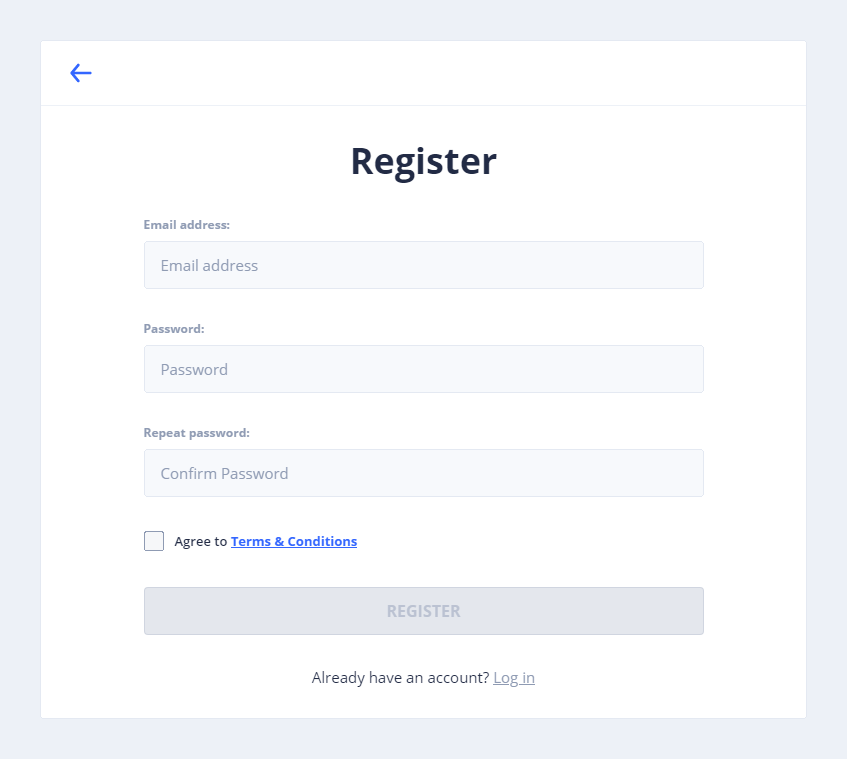
\includegraphics[width=.7\textwidth]{img/register.png}
    \caption{Registrierungs-Maske}
    \label{fig:registrierung}
\end{figure}


\section{Password-Vergessen}\label{sec:passwordVergessen}
Die Password-Vergessen-Funktion dient zum Zurücksetzen des Passwortes.
Möchte der Nutzer sein Password zurücksetzen und erneut Zugang zu seinem Account bekommen kann der Nutzer jederzeit seine Email in das Password-Vergessen-Feld eingeben.

\begin{figure}[h]
    \centering
    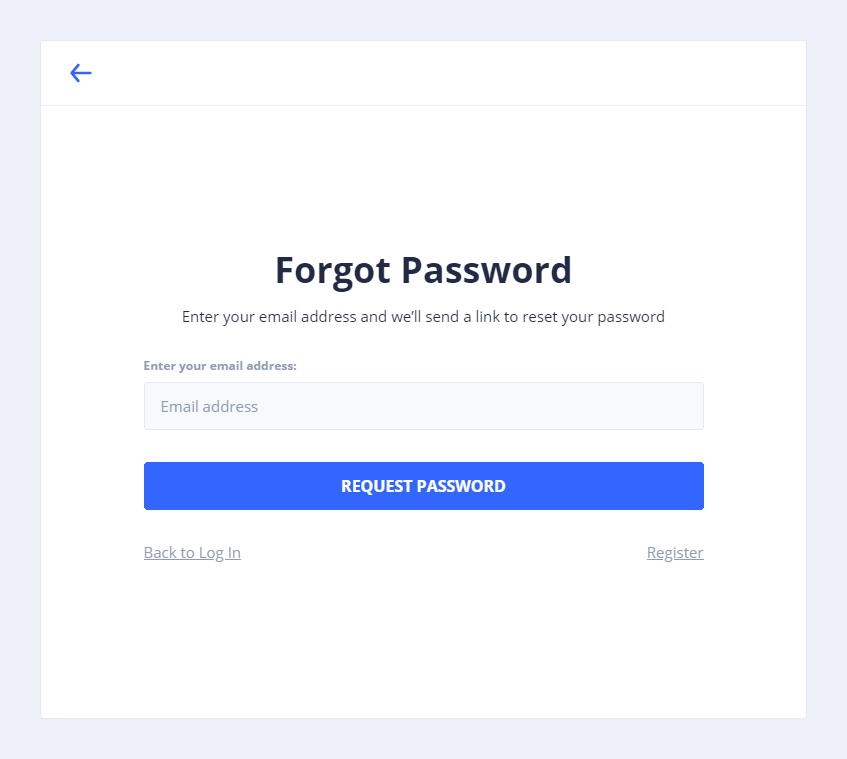
\includegraphics[width=.7\textwidth]{img/passwordReset.png}
    \caption{Password-Vergessen-Maske}
    \label{fig:passwordVergessen}
\end{figure}

Nachdem der Nutzer auf \enquote{Request Password} geklickt hat wird automatisch eine Email an die angegebene Email-Adresse gesendet.
Die Email enthält einen Link, mithilfe dem der Nutzer sein Passwort ändern kann.
Der Link leitet den Nutzer auf die in \autoref{fig:passwordVergessen} dargestellte Maske in der der Nutzer sein Passwort ändern kann.
Hat der Nutzer sein Passwort geändert wird der zu einem erneuten Login auf die Login-Maske geleitet.

Anzumerken ist, dass der Link zum Passwort ändern nur einmal gültig ist.
Sollte das Passwort bereits geändert worden sein, muss eine neue Email angefordert werden.
Dies verhindert, dass unberechtigte Personen die Email mitlesen können und das Passwort erneut ändern könn

% TODO: Muss man hier jede kleinigkeit schreiben? also das email auch wirklich eine email sein muss?


\begin{figure}[h]
    \centering
    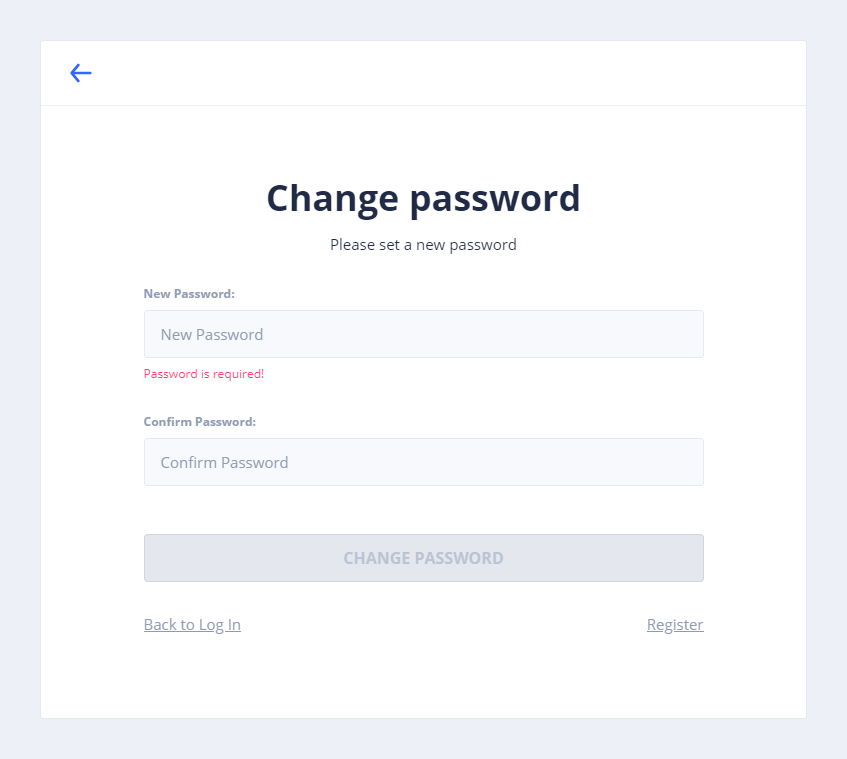
\includegraphics[width=.7\textwidth]{img/passwordReset2.png}
    \caption{Password-Aktualisieren-Maske}
    \label{fig:passwordVergessen2}
\end{figure}

% ..


\section{Dashboard}\label{sec:dashboard}
... siehe User Journey


\section{Karteikarten}\label{sec:Karteikarten} % TODO: Bilder
Index-Cards stellen eine Karteikarten-Funktion dar.
Im Nutzer-Interface werden Karten ähnlich zu einem realen Karteikasten hintereinander dargestellt.
Jede Karte zeigt zunächst die Frage an.
Solle man die Antwort zu der Frage nicht wissen oder sich kontrollieren wollen, kann man mithilfe des Pfeils im Eck einer jeden Karte die Antwort einblenden.
Anschließend können die Karten mit den Buttons am unteren Bildschirmrand als gewusst und nicht gewusst markiert werden.
Durch die Zahlen an diesen Buttons kann der Nutzer leicht ablesen, wie viele Karten der Nutzer bereits wusste.
Karten können aber auch durch einfaches ziehen der Karten zu gewusst oder nicht gewusst verschoben werden.
Dies erleichtert die Handhabung.

Wurden alle Karteikarten beantwortet bekommt der Student direkt Feedback, wieviel Prozent aller Fragen er richtig beantworten konnte.
% TODO: Zusätzlich bekommt er angezeigt, welche Karten er nocheinmal auffrischen sollte
% TODO: Erstellung


\section{TODOs}\label{sec:TODOs} % TODO:
TODOs stellen einen elementaren Bestandteil einer Ausbildung dar.
Schon in der Schule mussten Schüler eine Hausaufgabenheft oder Ähnliches führen um einen Überblick über ihre TODOs zu haben.
Auch im Studium gibt es Unzähliche TODOs, ...

TODOs können mithilfe des \enquote{Floating Action Button (FAB)} im rechten unterem Eck erstellt werden. % https://material.io/components/buttons-floating-action-button#usage
Fabs stellen die primäre Action einer Ansicht, die konstruktiv ist und zu dem Inhalt der Ansicht passt.
Inner


% TODO: Die Material Principien besser herausarbeiten  https://material.io/components/dialogs#usage
Nach dem Klick öffnet sich ein Modal, in dem alle relevanten Todos eingetragen werden können.
Todos zeichnen sich durch einen Titel und eine optionale Beschreibung, sowie eine optionale Deadline aus.
Sofern eine Deadline angegeben ist, wird dieses Todo in den Kalender über der Todo Übersicht dargestellt.
Je roter ein Tag ist, desto mehr Todos müssen an diesem Tag erledigt sein.
Der Kalender zeigt stets den Zeitraum zwischen Anfang des letzten Monates und Ende der nächsten zwei Monate  an.
% TODO: ?
Todos können schnell und einfach durch klicken auf die Checkbox vor einem Todo abgehackt werden.





% TODO: Das hier schreiben, wenn da tatsächlich was implementiert ist

% TODO: Kurs einschreibung, ...



\section{Files}
Die \enquote{Files}-Maske dient zur Verwaltung von Dokumenten.
% TODO: Das in Konzeption verschieben?
Momentan müssen Dokumente umständich an Studenten weitergegeben werden.
In der Regel werden Dokumente an die Studiengangsleiter geschickt, welche die Dokumente anschließend weiterverteilen.
Das Problem ist, dass zuerst die Email-Adressen dieser ausgetauscht werden müssen und diese einen zusätzlichen Aufwand haben.
So sind neue oder korrigierte Dokumente nur schwer auszutauschen.
Auch Dokumente, die während einer Vorlesung verteilt werden müssen, erzeugen eine Zeitdifferenz.
Dazu kommt, das dieser Workflow nicht immer gleich ist.
Oft bekommen verschiedene Schülter unterschiedliche Informationen.
In einigen Fällen wird auch Moodle für die Dateiablage verwendet.

Aus diesem Grund wird ein einheitliches System benötigt, in dem Dateien abgelegt werden können.

\begin{figure}[h] 
    \centering
    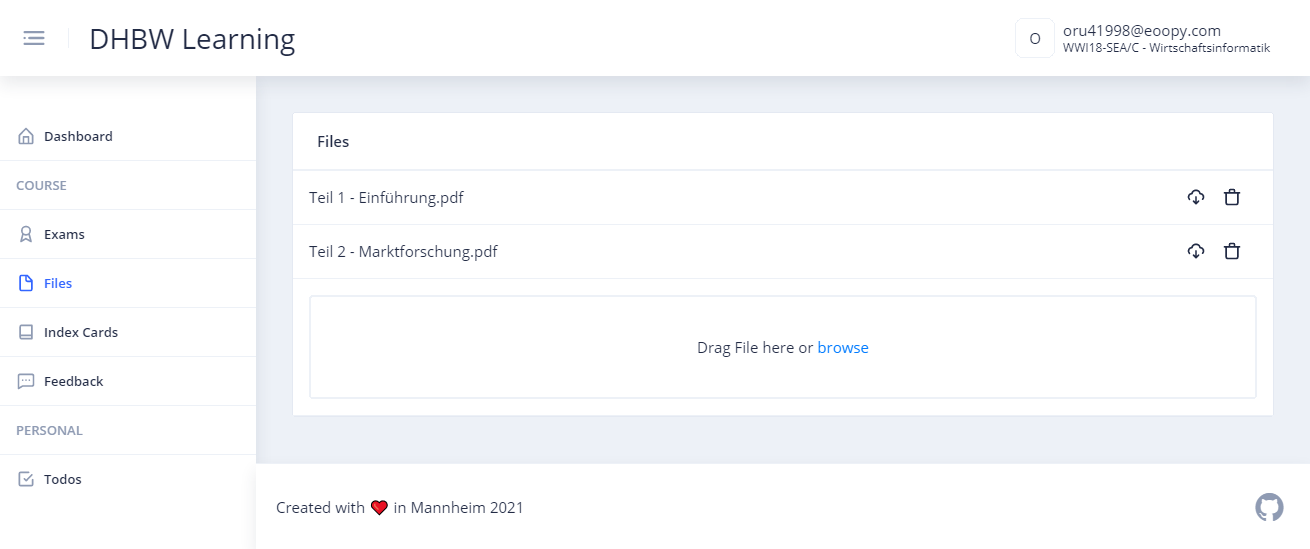
\includegraphics[width=\textwidth]{img/Files.png}
    \caption{Files-Maske}
    \label{fig:files}
\end{figure}

Das in \autoref{fig:files} dargestellte Datenmanagementsystem erleichtert dies, da Dokumente für einen Kurs hochgeladen werden können.
Dokumente können mithilfe des \enquote{browse}-Button hochgeladen werden.
Dafür öffnet sich ein Fenster, in dem beliebig viele Dateien für den Upload hochgeladen werden.
Zur einfacheren Nutzung können optional auch Dateien direkt aus dem Explorer in das Fenster gezogen werden.

Anschließend werden die Dateien hochgeladen.
Ein Fortschrittsbalken zeigt dabei stets den aktuellen Upload-Fortschritt an.
Anschließend können die Dokumente von allen Studenten heruntergeladen werden.
% TODO: Buttons rechts?

% TODO: Müssen die Toasts auch erklärt werden?

Bei der Nutzung des Dateisystems ist darauf zu achten, dass aus Speichergründen nicht alle Dateien antizipierend heruntergeladen werden können.
Dies würde es ermöglichen Geräte von Studenten zu überfordern.
Besonders Mobilgeräte besitzen noch einen begrenzten Speicher.
Aus diesem Grund muss während der Benutzung auf eine Internetverbindung geachtet werden.
Offline können nur die existierenden Dateien angezeigt werden, aber weder neue hochgeladen noch bestehende heruntergeladen werden.


Aus technischer Sicht werden mehrere Schritte unternommen, um die Dateiablage zu ermöglichen.
Sobald Dateien ausgewählt wurden oder Dateien in das Fenster gezogen wurde wird der Upload dieser zu FireStorage angestoßen.
Dabei handelt es sich um einen Bucket-basierte Speicherlösung ähnlich zu AWS S3. % TODO: Das genauer erklären?
Während des Uploads wird der Zustand überwacht, wieviel der Datei bereits übertragen werden konnte.
Dieser Wert wird automatisch in den Fortschrittsbalken weitergeleitet, welcher sich dadurch reaktiv aktualisiert.


Konnte der Upload erfolgreich durchgeführt werden wird der Fortschrittsbalken grün und eine Benachrichtigung informiert informiert, dass die Datei erfolgreich hochgeladen werden konnte.
Im Hintergrund wird anschließend ein Datenbankeintrag getätigt, ab welchem Zeitpunkt andere Nutzer auf die Datei zugreifen können.

Wird eine Datei gelöscht wird der gleiche Vorgang rückwärts durchgeführt.
Das heißt, zuerst wird der Datenbankeintrag gelöscht, wodurch Studenten nicht mehr darauf zugreifen können.
Anschließend wird die eigentliche Datei aus dem Bucket-Speicher gelöscht.

% TODO: uuidv4 erklären?#
% TODO: Disposition header erklären wegen datei namen und sicherheit cross domain?

% TODO: Technische Implementierung




% TODO: Logout



% TODO: Konform zum Müll Artikel 17


\section{Feedback}
% TODO: Das in die Anforderungen packen + die Anwendung in die Abgrenzung zu anderen Softwares packen + Mit Personas verknüpfen
Die Feedback-Maske dient dazu, einem Dozenten eine unmittelbare Rückmeldung zu geben, wodurch Dozenten jederzeit ihren Vorlesungsstil anpassen können.
Gegenwärtig existieren Umfragen am Ende jedes Semesters, in dem Studenten die Vorlesung bewerten können.
Problematisch ist, dass diese Umfragen erst am Ende eines Semesters durchgeführt werden.
Das bedeutet, dass unter Umständen eine ganze Vorlesungsreihe suboptimal durchgeführt wird.
Dazu kommt, dass es an der DHBW einen stetigen Ausstausch an Dozenten gibt.
Neue Dozenten haben noch keine Erfahrung im Halten von Vorlesungen.
Viele der Dozenten fragen bereits während der ersten Vorlesungen um Feedback.
Aus diesem Grund wird eine anonyme Plattform benötigt, bei dem kurzzeitig Feedback gegeben werden kann.

Im Vergleich zu den Umfragen am Ende eines Semesters werden die Umfragen in der Anwendung kurz gehalten.
Dies geht daraus hervor, dass es als eine schnelle Feedbackmöglichkeit gedacht ist und eine kurze Umfrage die Change erhöht, dass das Feedback ausgefüllt wird.
Um neutrale Feedbacks zu vermeiden gibt es eine grade Anzahl an Auswahlmöglichkeiten. 



% TODO: Sollte Feedback pro gehaltene Vorlesung sein? -> Einzelne Bereiche einer Vorlesung vertiefen
% Hier kann man vielleicht auch was aus BI sagen, mit Identifikationsfragen, ...
% Lange Umfragen sind blöd



% TODO: Aspekte Learning Analytics
% Das steht schon im Referenzdokument.
% Dann kamm man sagen, Learning Awareness, Privacy Awarness ...  konzentieren wir uns drauf

% TODO: Quotas erwähnen?



\section{Exams}
Als Studenten konnten wir ein weiteres Problem mit der aktuellen Informationsversorgung identifizieren.
Momentan herrscht eine große Unklarheit über Prüfungsleistungen.
Teilweiße werden die Prüfungsleistungen in den Vorlesungen angekündigt, manche in Moodle und wieder andere werden in einem Google Calendar eingetragen.
Außer einem Datum sind oft keine weiteren Informationen festgesetzt.
Stattdessen werden diese mündlich in den Vorlesungen bekanntegegeben.
Besonders für Studenten die Aufgrund von Krankheiten oder, in der Zeit von Online-Vorlesungen, Internetverbindugnsprobleme besitzen ist dies problematisch, wenn sie diese Informationen nicht mitbekommen.

Dazu kommt, dass besonders bei Portfolioprüfungen, Prüfungen nicht aus einer einzelnen, sondern aus mehreren Leistungen bestehen.
Ein Beispiel ist die Erstellung einer Präsentation, bei die nicht nur der Vortrag, sondern auch das Begleitmaterial bewertet wird.

Aus diesem Grund können in der Anwendungen Informationen über Klausuren verwaltet werden.
% TODO: 
Jede Prüfungsleistung besitzt einen Titel und einer Beschreibung, in der beschrieben werden kann, was die Aufgabe ist.
Außerdem wird das Abgabedatum in einem Kalender zur einfacheren Übersicht dargestellt.
Zusätzlich werden alle wichtigen Informationen, wie Räume oder zugelassenen Hilfsmittel dargestellt.



% Fazit und Ausblick
% !TEX root =  master.tex
\chapter{Zusammenfassung}

\section{Fazit} % TODO: Das auch dann nochmal anpassen
In dieser Arbeit wurde eine Webanwendung erstellt, die Studenten und Dozenten im Hochschulkontext unterstützt.
Dafür wurden zuerst die funktionalen und nicht-funktionalen Anforderungen festgelegt.
Anschließend wurde ein Konzept ausgearbeitet, welches anschließend in einer Webanwendung umgesetzt wurde.
% TODO:



\section{Ausblick}
Wir sehen mit der bereits entwickelten Anwendung bereits ein großes Potenzial, welches die Organisation und den Klausurerfolg steigern kann.
Dennoch ist der Funktionsumfang der Anwendung recht limitiert.
In zukünftigen Implementierungen sehen wir besonders großes Potenzial in den folgenden Bereichen:
\begin{itemize}
    \item Live-Chat\\
        Wenn Fragen während des Lernens entstehen müssen gegenwärtig weitere Kanäle verwendet werden.
        So werden beispielsweise Google-docs-Dokumente geteilt, in den Studenten Fragen eintragen können.
        Dozenten schauen in diese Dokumente und schreiben ihre Antworten zu diesen.
        Besser wäre stattdessen ein Live-Chat, in dem alle Teilnehmer und Dozenten zu einer Vorlesung direkt befragt werden können und so das Zusammenarbeit gefördert wird.
        % TODO: Da kann man ja nebulars chat modul darstellen
    \item Import\\
        Eine weitere hilfreiche Funktion wäre der Import existierender Daten.
        So wäre es praktisch existierende Informationen aus Moodle oder Google Calendar zu importieren.
        Dadurch wäre der Umstieg in die Anwendung einfacher. 
    \item Analysen\\
        Damit sich Dozenten einen besseren Überblick über den Kurs und den Lernfortschritt machen wären auch Analysen sinnvoll.
        Beispielsweise könnte die Anwendung um Umfragen oder indirekte Datenerhebungsmethoden ergänzt werden.
\end{itemize}

% TODO: Bewertungen
% TODO: Internationalisierung

%%%%%%%%%%%%%%%%%%%%%%%%%%%%%%%%%%%

\initializeAppendix

%%%%%%%%%%%%%%%%%%%%%%%%%%%%%%%%%%%
% ANHÄNGE
%
% @stud: einzelne Anhänge bearbeiten und eigene Anhänge hier einfügen 
%
% % !TEX root =  master.tex
\chapter{Beispiel-Anhang: Testanhang}
Anh\"ange\index{Anhang} werden am Ende Ihrer Arbeit vor dem Literaturverzeichnis und dem Index eingef\"ugt.

\section{Abschnitt im Anhang}

\lipsum

%%%%%%%%%%%%%%%%%%%%%%%%%%%%%%%%%%%

\singlespacing

%%%%%%%%%%%%%%%%%%%%%%%%%%%%%%%%%%%
% LITERATURVERZEICHNIS
% 
% @stud: Literaturverzeichnis in Datei bibliography.bib anpassen 
%
\initializeBibliography
%%%%%%%%%%%%%%%%%%%%%%%%%%%%%%%%%%%

\addcontentsline{toc}{chapter}{Index}
\printindex

\end{document}
